\documentclass[a4paper,12pt, master]{etf}

\usepackage[intlimits]{amsmath}
\usepackage{amsmath, amsfonts, amssymb, graphicx}

\usepackage[serbian]{babel}
\usepackage[T1]{fontenc}
\usepackage[utf8]{inputenc}
\usepackage{graphicx}

\addto\captionsserbian{\renewcommand{\bibname}{Literatura}}

\title{Implementacija vremenske sinhronizacije u Namenskim ra\v{c}unarskim sistemima}
\author{Lazar Caković}
\indeks{3083/2016}
\date{septembar 2018.}
\mentor{Prof\. dr Lazar Saranovac}
\predmet{}

\begin{document}

	\maketitle

	\tableofcontents

	\listoffigures

	\newpage

	\chapter{Apstrakt}

	\newpage

	\chapter{Uvod}

	Vremenska sinhrnozacija igra fundamentalnu ulogu u svakoj mre\v{z}i, ali je ipak naj\v{c}e\v{s}\'{c}e
	dodata kao naknadna funkcionalnost. Ipak, mo\v{z}e zna\v{c}iti razliku izmedju egzaktnog
	odredjivanja gre\v{s}aka unutar sistema, u ta\v{c}nim vremenskim trenucima, i nepostojanje ideje
	za\v{s}to se server pona\v{s}a onako kako nije predvidjeno. (``Time synchronization
	serves a fundamental role in any network, but it's too often added as an afterthought.
	However, it can mean the difference between correctly troubleshooting a conflict in
	minutes and having no idea why the server is figuratively on fire.'') Za finansijske i
	nau\v{c}ne institucije, vremenska sinhronizacija mora biti ta\v{c}na na milijarditi, ili nekad na
	trilioniti deo sekunde, medjutim sve vi\v{s}e komercijalnih i industrijskih organizacija se
	sve vi\v{s}e zala\v{z}u za ideju da preciznost vremenske sinhronizacije bude u sub-milisecond
	opsegu.	Za\v{s}to nije dovoljno da sse uredjaji inhronizuju preko javno dostupnog NTP
	protokola. Na\v{z}alost, ka\v{s}njenje postoji svugde, i prosto je nemogu\'{c}e posti\'{c}i savr\v{s}enu
	sinhrnoizaciju. Brzina svetlosti je brza, u vakumu, foton moze napraviti krug oko zemlje
	vi\v{s}e od 7 puta u sekundi, iako putuje aproksimativno 31\% sporije kroz obi\v{c}nu opti\v{c}ku
	mre\v{z}u, lako se mo\v{z}e preneti jedan bit informacije preko pola sveta za manje od desetine
	sekunde. Ali, svi znamo da idealan svet ne postoji. Dodati svi\v{c}eve (switches),
	rutere, i ostalu mre\v{z}nu infrastrukturu, i ta desetina sekunde se uve\'{c}a nekoliko puta. Bez
        specijalizovane opreme, na\v{s}a mre\v{z}a lako mo\v{z}e dodati ka\v{s}njenje \v{c}ak i ve\'{c}e od
	sekunde. Jo\v{s} ve\'{c}a briga je sinhronizacija razli\v{c}itih uredjaja unutar iste mre\v{z}e.

	Sinhronizacija postaje neophodna kada su uredjaji koji rade zajedno na odredjenoj
	udaljenosti moraju raditi u vezi jedni sa drugima. U ovim scenarijima, lokalni sat, ili
	Master Sat, sinhronizuje sve uredjaje u istom sistemu sa tim satom. Zbog ove potrebe za
	sinhronizacijom, IEEE 1588 standard je objavljen kao standardni protokol 2002. godine.
	Iako su dva sata unutar uredjaja pode\v{s}eni da rade na istoj frekvenciji, ne postoji garancija
	da \'{c}e ostati sinhronizovani. Upravo zbog ovoga proces sinhronizacije je neprekidan. Nekoliko
	faktora mo\v{z}e uticati na to da dva identi\v{c}na sata izgube sinhronizaciju. Razlozi mogu biti
	razli\v{c}iti, kao na primer razlika u temperaturi, starosti uredjaja, kao i frekvenciji na kojoj
	uredjaji rade, koja mo\v{z}e uticati na kvalitet sinhronizacije. Upravo iz ovih razloga je i
	nastala potreba za sinhronizacijom uredjaja.

	\section{Network Time Protocol}

	NTP, ili Network Time Protocol, je \v{s}iroko prihva\'{c}en kao sredstvo za \v{c}uvanje vremena na
	mre\v{z}i, i trenutno je u upotrebi \v{c}etvrta verzija samog protokola. Hijerarhijski sistem ima
	razli\v{c}ite slojeve koji se nazivaju STRATA (strata eng.). Statum 0
	uredjaji su u samom vrhu i uklju\v{c}uju atomske satove, kao one koji se nalaze u GNSS
	satelitima.	Stratum 1, ili primarni vremenski server, svaki od njih ima jedan na jedan
	direktnu konekciju sa Stratum 1 satom, i posti\v{z}u sinhronizaciju red mikrosekunde sa Stratum
	0 satovima, i povezuju se na ostale Stratum 1 severe za brzu proveru satova i \v{c}uvanje
	podataka. Stratum 2 serveri se mogu povezivati na vi\v{s}e primarnih vremenskih servera kako
	bi se postigao ve\'{c}i level sinhronizacije i pobolj\v{s}ala preciznost, i tako dalje. NTP
	podr\v{z}ava maksimum od 15 strata uredjaja, ali svaki strata uredjaj unosi malu gre\v{s}ku u
	sinhronizaciji sa Stratum 0 uredjajima.

	64-bitni vremenski \v{z}ig je trenutno implementiran kako bi se podelio u dva 32-bitna dela.
	\begin{itemize}
		\item Prva polovina broji broj sekundi do ne\v{s}to preko 136 godina.
		\item Druga polovina predstavlja deo sekunde do razmere pikosekunde
	\end{itemize}

	Predlo\v{z}ena je promena na 128-o bitne vremenske \v{z}igove u NTPv4 protokolu, i trebalo bi da
	pove\'{c}a vremensku razmeru na ne\v{s}to manje od 600 milijardi godina, pri \v{c}emu bi vremenska
	rezolucija bila manja od femtosekunde.

	\section{Precision time protokol}

	PTP, ili Precision time protokol, je jo\v{s} jedan standard za sinhronizaciju vremena preko
	mre\v{z}e, ali umesto sinhronizacije reda veli\v{c}ine milisekunde, PTP mre\v{z}e mogu da postignu
	sinhronizaciju reda veli\v{c}ine nanosekunde, ili \v{c}ak pikosekunde. Za ve\'{c}inu komercijalnih i
	industrijskih aplikacija, NTP je vi\v{s}e nego precizan, ali ukoliko je potrebna ta\v{c}nija
	sinhronizacija i ta\v{c}nije obele\v{z}avanje vremena, potrebno je migrirati sistem na PTP.

	Zbog \v{c}ega je PTP toliko ta\v{c}an? Koristi obele\v{z}avanje paketa hardverskim vremenskim
	\v{z}igovima, umesto softverskih, i kao svaki fini nau\v{c}ni instrument, PTP oprema je
	specijalizovana za samo jednu specijalizovanu svrhu: o\v{c}uvanje sinhronizacije izmedju
	uredjaja. Samo iz ovih razloga, PTP mre\v{z}e imaju mnogo ta\v{c}niju vremensku rezoluciju, i ne
	kao NTP uredjaji, PTP uredjaji ce ustvari uklju\v{c}iti vreme koje svaka od sinhronizacionih
	poruka provede u svakom od uredjaja, \v{s}to uklju\v{c}uje i ka\v{s}njenje u uredjaju.

	Svaka od PTP razmena uklju\v{c}uje seriju od 4 poruke koje se razmenjuju izmedju master-a i
	slave-a:
	\begin{itemize}
		\item Inicijalna sinhronizaciona poruka od mastera ka slejvu {Sync message}
		\item Poruka koja prati sinhronizacionu poruku od mastera ka slejvu {Follow\_up message}
		\item Poruka sa zahtevom za odredjivanje ka\v{s}njenja od slejva ka masteru {Delay\_Req
		message}
		\item Finalni odgovor sa ka\v{s}njenjem od mastera ka slejvu {Delay\_Resp message}
        \end{itemize}

	Ova razmena pru\v{z}a \v{c}etiri razli\v{c}ita vremena:
	\begin{itemize}
		\item T1 -> vreme kad master posalje inicijalnu sinhronizacionu poruku
		\item T2 -> vreme kad slejv dobije inicijalnu sinhronizacionu poruku
		\item T3 -> vreme kad slejv posalje poruku sa zahtevom za ka\v{s}njenjem
		\item T4 -> vreme kad master dobije zahtev za ka\v{s}njenjem
        \end{itemize}

	Master \v{s}alje sva 4 vremenska \v{z}iga ka slejvu tokom faze odgovora na zahtev za ka\v{s}njenjem,
	i slejv mo\v{z}e sa tim vremenima da izra\v{c}una ka\v{s}njenje po mre\v{z}i izmedju mastera i slejva u
	oba smera. Imaju\'{c}i specijalizovani hardver koji mo\v{z}e da uhvati vremena lokalnog sata,
	slejv uredjaji mogu izbe\'{c}i dodatno ka\v{s}njenje koje je uslovljeno lokalnim operativnim
	sistemom.

	NTP mre\v{z}e imaju dodatno ka\v{s}njenje i manju preciznost jednostavno zbog toga \v{s}to su
	softverski bazirane, i svi zahtevi za vremenima moraju da \v{c}ekaju na lokalni operativni
	sistem. Za ve\'{c}inu kompanija, NTP pru\v{z}a dovoljno ta\v{c}nu rezoluciju vrmena kako bi se re\v{s}ili
	svi konflikti u dogledno vrmene, dok neke organizacije zahtevaju dosta ve\'{c}i nivo
	sinhronizacije.

	IEEE 1588 obezbedjuje sinhronizaciju dva sata u istoj mre\v{z}i koja je otporna na gre\v{s}ke.
	Takodje, koristi se veoma mali opseg frekvencija, procesna mo\'{c}, ali i pode\v{s}avanje samog
	protokola. IEEE 1588 standard posti\v{z}e sve ovo koriste\'{c}i protokol preciznog vremena
	(Precision Time Protocol), ili PTP\@. Vremenski protokol koji se koristi sinhronizuje dva sata na
	mre\v{z}i pode\v{s}avaju\'{c}i satove ka ``najkvalitetnijem'' satu. IEEE 1588
	defini\v{s}e ospege vrednosti za standardan set karakteristika satova. Algoritam najboljeg
	sata, BMC algorithm, odlu\v{c}uje koji sat na mre\v{z}i je ``najkvalitetniji'', odnosno koji sat na
	mre\v{z}i je najta\v{c}niji, i najbolji kako bi se ostali uredjaji sinhronizovali na njega. BMC
	algoritam onda sinhronizuje sve ostale satove (slave clocks) sa ovim satom na mre\v{z}i.
	Ukoliko se BMC (Best Master Clock) ukloni iz mre\v{z}e, ili BMC algoritam odlu\v{c}i da taj sat
	nije vi\v{s}e najta\v{c}niji, algoritam redefini\v{s}e novi ``najkvalitetniji'' sat, i prilagodi
	vremena ostalih satova u skladu sa tim. Nije potrebno da se administrator mre\v{z}e uklju\v{c}uje
	u bilo kom trenutku kako bi se promenio najbolji sat u mre\v{z}i, zbog toga \v{s}to je ovaj
	algoritam otporan na gre\v{s}ke.

	U ovu svrhu koristi se Bidirekciona multikast komunikacija (Bidirectional Multicast Communication)
	 od strane slave uredjaja kako bi se sinhronizovali na najbolji sat, IEEE 1588 grandmaster clock.
	``Sync'', Sinhronizacioni paket sadr\v{z}i vremenski \v{z}ig najboljeg sata, koji predstavlja
	ta\v{c}no vreme kada je paket poslat sa grandmaster clock-a. ``Follow up'', Prate\'{c}i paket
	takodje mo\v{z}e biti poslat sa grandmaster sata, koji sadr\v{z}i vremenski \v{z}ig ``Sync''
	(sinhronizacionog) paketa. Ovakav princip razmene podataka omogu\'{c}ava ta\v{c}an vremenski
	\v{z}ig sinhronizacionog paketa koji je prosledjen sa grandmaster sata. Takodje, postoje
	slu\v{c}ajevi u kojima se ne otkriva ta\v{c}no vreme slanja paketa, zbog odredjenih smetnji na
	mre\v{z}i. Ovo je omogu\'{c}eno kroz Collision detection i Random Back-off
	mehanizam u Ethernet/IP komunikaciji. Samo onda kad je paket kompletno poslat, nemogu\'{c}e
	je promeniti sadr\v{z}aj paketa.

	Postoji nekoliko faktora koji mogu uticati na egzaktnost sinhronizacije izmedju dva
	uredjaja unutar IEEE 1588 mre\v{z}e. Promene frekvencije na uredjaju koji daje ta\v{c}no vreme,
	koje se mo\v{z}e desiti izmedju dva sinhronizaciona paketa ``Sync'', mogu uzrokovati da se
	izgubi sinhronizacija sa ostalim uredjajima u istom sistemu. Kako bi se predupredila
	svaka mogu\'{c}nost za gubljenje sinhronizacije, mogu se koristiti uredjaji sa veoma velikom
	stabilno\v{s}\'{c}u, kao i da se skrati vreme izmedju razmene sinhronizacionih paketa. Kako bi
	se jo\v{s} vi\v{s}e unapredila sinhronizacija, mogu se koristiti druge vrste oscilatora u
	uredjajima, narocito Temperature Controlled Crystal Oscillators (TXCOs) i Oven Controlled Crystal
	Oscillators (OCXOs). Rezulucija sata mo\v{z}e uticati na preciznost vremenskih \v{z}igova unutar
	sinhronizacionih paketa. D\v{z}iter (Jitter) iz susednih uredjaja u mre\v{z}i, kao sto su habovi i
	svi\v{c}evi (hubs and switches), takodje mogu uticati na preciznost sinhronizacije. Kvalitet IEEE 1588
	mre\v{z}nog sistema i kako je pode\v{s}en mo\v{z}e takodje uticati na kvalitet sinhronizacije. Kako bi
	se podesio sistem sa \v{s}to boljom sinhronizacijom, mora se napraviti kompromis izmedju
	egzaktnosti sinhronizacije, cene, kao i razdaljine izmedju uredjaja u sistemu. Za sporije
	dogadjaje unutar sistema koji ne zavise od vremena, standardna NTP sinhronizacija preko
	interneta, koja daje sinhronizaciju na nivou milisekunde, zadovoljava sve potrebe. IEEE
	1588 je i dalje izvanredna alternativa za sisteme koji zahteva sinronizaciju na nivou ispod
	mikroseunde.

	Precizna sinhronizacija se mo\v{z}e iskoristiti u slede\'{c}im aplikacijama:
	\begin{itemize}
		\item Telekomunikacije
		\item Energetska postrojenja
		\item Industrijska automatizacija
		\item Testiranje i merenja
		\item Robotska kontrola
	\end{itemize}

	\newpage

        \chapter{Protokol}

        U ovom odeljku \'{c}e biti dat pregled konceptualnih modela Ethernet komunikacije, kao i obja\v{s}njenje
        celog PTP protokola. Na po\v{c}etku \'{c}e biti predstavljen OSI konceptualni model, nakon njega TCP/IP
        model, i na kraju sam protokol koji je kori\v{s}cen. Ovaj pregled je dat u svrhu dobijanja slike o tome
        koliko je kompleksan sam stek (\#\# [lazarc] stack) koji se koristi, kao i da se dobije slika o nekim
        delovima koji \'{c}e kasnije biti spominjani.

	\section{OSI model}

	Open Systems Interconnection model (OSI model) je konceptualni model koji karakteri\v{s}e i
	standardizuje komunikacione funkcije u telekomunikacionim ili kompjuterskim sistemima, i
	to bez obzira na unutra\v{s}nju strukturu uredjaja ili njihovu tehnologiju. Cilj ovog modela
	je da se postigne kompatibilnost razli\v{c}itih komunikacionih sistema sa standardnim
	protokolima komunikacije. OSI model razdvaja komunikacione sisteme u apstraktne slojeve.
	Originalna verzija modela ima sedam slojeva.

	Sloj unutar modela slu\v{z}i sloj iznad njega, i koristi sloj ispod njega u hijerarhiji. Na
	primer, sloj koji posti\v{z}e komunikaciju preko mre\v{z}e bez gre\v{s}aka, slu\v{z}i aplikacijama iznad
	koje ga koriste, i to dok poziva jednostavne funkcije za prijem i predaju paketa na mre\v{z}i.
	Dve instance istog sloja su vizualizovane tako \v{s}to su povezane horizontalno u istom sloju.

	Ovaj model je proizvod Open Systems Interconnection projekta u International Organization
	for Standardization (ISO), i ima oznaku ISO/IEC 7498-1.

        \begin{figure}[htb]
                \centering
                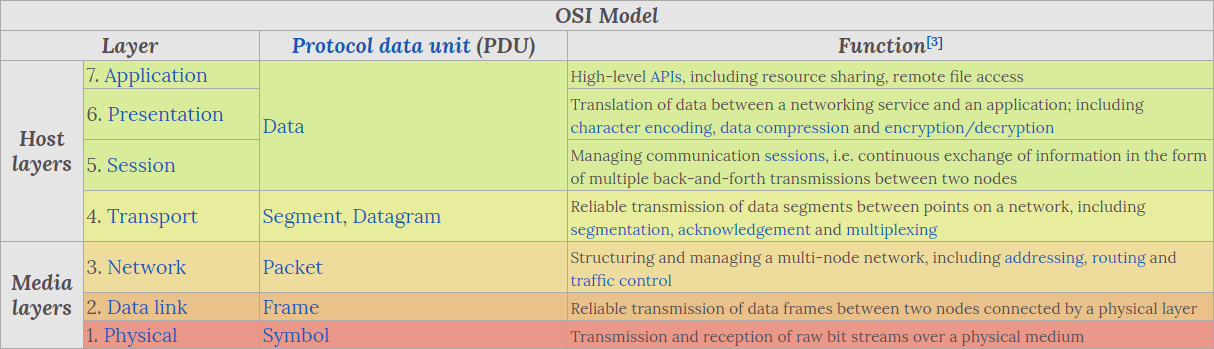
\includegraphics[scale=.43]{../pic/osi_model.png}
                \caption{Prikaz svih slojeva unutar OSI modela komunikacije}
                \label{fig:osi_model}
        \end{figure}

	Na svakom nivou N, dva entiteta na komunikcionim uredjajima razmenjuju jedinice protokola
	(PDU - protocol data units) pomocu sloja N protokola. Svaki PDU sadrzi podatke od interesa
	(payload) (SDU - service data unit), zajedno sa zaglavljima koji odgovaraju protokolu.

	Obrada podataka izmedju dva uredjaja koji su OSI-kompatibilni se odvija u slede\'{c}im
	koracima:
	\begin{itemize}
		\item Podaci koji se prenose se formiraju na najvi\v{s}em sloju u uredjaju koji predaje
		podatke na mre\v{z}i (sloj N) u jedinicu protokola (PDU).
		\item PDU se prosledjuje sloju N-1, gde je poznat kao SDU.
		\item Na sloju N-1 se na SDU dodaju zaglavlja, na osnovu \v{c}ega se formira PDU za sloj
		N-1. Nakon \v{c}ega se prosledjuje na sloj N-2.
		\item Ovaj postupak se ponavlja sve dok se ne dostigne najni\v{z}i sloj u modelu, nakon
		\v{c}ega se podaci prenose ka uredjaju koji prima podatke.
		\item Na strani prijemnog uredjaja se podaci prenose od najni\v{z}eg sloja u modelu, do
		najvi\v{s}eg, gde se serije SDU struktura uspe\v{s}no obradjuju, pri \v{c}emu se skidaju zaglavlja
		sa svakog sloja, dok se ne dostigne najvi\v{s}i sloj u modelu, nakon \v{c}ega su dostupni
		sirovi podaci.
	\end{itemize}

	\subsection{Sloj 1: Fizi\v{c}ki sloj (Physical Layer)}

	Fizi\v{c}ki sloj je odgovoran za prenos i prijem nestrukturiranih sirovih podataka izmedju
	uredjaja i fizi\v{c}kog medijuma za prenos. On pretvara digitalne bitove u elektri\v{c}ne, radio
	ili opticke signale. Specifikacije sloja defini\v{s}u karakteristike poput nivoa napona,
	fizi\v{c}ke brzine prenosa podataka, maksimalne udaljenosti prenosa i fizi\v{c}kih konektora. Ovo
	uklju\v{c}uje raspored pinova, napona, linijske impedanse, specifikacije kablova, vremenskih
	signala i frekvencije za be\v{z}i\v{c}ne uredjaje. Kontrola brzine bitova se vr\v{s}i na fizi\v{c}kom
	nivou i mo\v{z}e definisati na\v{c}in komunikacije kao simpleks, polu dupleks ili dupleks
	komunikaciju. Komponente fizi\v{c}kog sloja mogu se opisati u smislu topologije mre\v{z}e.
	Bluetooth, Ethernet i USB, sve imaju specifikacije za fizi\v{c}ki sloj.

	\subsection{Sloj 2: Sloj veze (Data Link Layer)}

	Sloj veze podataka obezbedjuje prenos podataka izmedju dva \v{c}vora u komunikaciji - vezu
	izmedju dva direktno povezana uredjaja na mre\v{z}i. Ovaj sloj otkriva i eventualno ispravlja
	gre\v{s}ke koje se mogu javiti u fizi\v{c}kom sloju. On defini\v{s}e protokol za uspostavljanje i
	prekid veze izmedju dva fizi\v{c}ki povezana uredjaja. Takodje, defini\v{s}e protokol za kontrolu
	protoka izmedju njih.

	IEEE 802 standard deli sloj veze na dva podsloja:
	\begin{itemize}
		\item \textbf{Kontrola pristupa medijumu (MAC - Medium access control):}
		odgovorna je za kontrolu na\v{c}ina na koji uredjaji na mre\v{z}i dobijaju pristup medijumu i
		dozvolu za prenos podataka.
		\item \textbf{Kontrola logicke veze (LLC - Logical link control):}
		odgovorna je za identifikaciju i enkapsulaciju slojeva mre\v{z}nog protokola, i kontrolu
		gre\v{s}aka i sinhronizaciju paketa koji se \v{s}alju.
	\end{itemize}

	MAC i LLC slojevi IEEE 802 mre\v{z}nog standarda kao \v{s}to su 802.3 Ethernet, ili 802.11 Wi-Fi su
	slojevi veze (data link layer).

	Point-to-Point Protocol (PPP) - je protokol sloja veze koji radi na nekoliko razli\v{c}itih
	fizi\v{c}kih slojeva, kao \v{s}to su sinhrone ili asinhrone serijske linije.

	\subsection{Sloj 3: Mre\v{z}ni sloj (Network Layer)}

	Mre\v{z}ni sloj obezbedjuje funkcionalno i proceduralno sredstvo prenosa sekvenci podataka
	promenljive du\v{z}ine, koji se nazivaju jo\v{s} i paketi, od jednog \v{c}vora do drugog, poveznih u
        ``razli\v{c}ite mre\v{z}e''. \#\# [lazarc] [prevod] \#\# Mre\v{z}a je medijum na koji mo\v{z}e biti
        povezano vi\v{s}e \v{c}vorova, u kom svaki \v{c}vor ima adresu i koji dozvoljava \v{c}vorovima povezanim
        sa njim da prenose poruke ka ostalim \v{c}vorovima, i to samo daju\'{c}i sadr\v{z}aj poruke i adresu
        \v{c}vora na koji poruka treba da bude dostavljena, omogucavaju\'{c}i mre\v{z}i da nadje na\v{c}in da
        isporu\v{c}i poruku odredi\v{s}nom \v{c}voru, eventualno ga usmeravaju\'{c}i kroz sredi\v{s}nje
        \v{c}vorove (uredjaje koji su izmedju dva uredjaja koji poku\v{s}avaju da komuniciraju). Ako je poruka
        prevelika da bi se prenela sa jednog uredjaja na drugi samo kori\v{s}\'{c}enjem sloja veze (Data Link
        Layer), mre\v{z}a mo\v{z}e preneti podatke tako \v{s}to \'{c}e ih podeliti u nekoliko delova na jednom
        uredjaju, poslati delove nezavisno, i onda spojiti delove na drugom uredjaju. Pri \v{c}emu mo\v{z}e, iako
        nije uvek potrebno, prijaviti gre\v{s}ke u isporuci.

	Isporuka poruka na mre\v{z}nom sloju nije garantovano pouzdana. Mre\v{z}ni sloj mo\v{z}e pru\v{z}iti
	pouzdanu isporuku poruka, ali nije obavezno da to mora biti ispunjeno.

	Neki broj protokola koji upravljaju slojevima, imaju funkciju koja je definisana u aneksu
	upravljanja, ISO 7498/4, i pripadaju mre\v{z}nom sloju. Oni uklju\v{c}uju protokole rutiranja,
	upravljanja grupom sa vi\v{s}e uredjaja, informacije o mre\v{z}nom sloju, o gre\v{s}kama, kao i
	dodeljivanje adresa mre\v{z}nog sloja medju uredjajima. Ustvari, to je funkcija podataka koji
	se prenose uz pomo\'{c} protokola, \v{s}to ih \v{c}ini da pripadaju mre\v{z}nom sloju, a ne protokolu.
	\#\# [lazarc] poslednja	recenica [prevod] \#\#

	\subsection{Sloj 4: Transportni sloj (Transport Layer)}

	Transportni sloj obezbedjuje funkcionalno i proceduralno sredstvo prenosa sekvenci podataka
	promenljive du\v{z}ine od predajnog do prijemnog uredjaja, uz odr\v{z}avanje kvaliteta.

	Transportni sloj kontroli\v{s}e pouzdanost date konekcije kroz kontrolu protoka,
	segmentaciju/desegmentaciju i kontrolu gre\v{s}aka. Neki protokli su orjentisani na stanje
	mre\v{z}e, a neki na konekciju u mre\v{z}i. \#\# [lazarc] [prevod] \#\# Ovo zna\v{c}i da Transportni
	sloj mo\v{z}e da prati segmente i ponovo prenese one koji nisu isporu\v{c}eni prijemnom uredjaju.
	Transportni sloj takodje omogu\'{c}ava i potvrdu uspe\v{s}nog prenosa podataka i \v{s}alje naredne
	podatke ako nije do\v{s}lo do gre\v{s}ke prilikom prenosa. Transportni sloj formira i segmente
	koji su primljeni iz vi\v{s}ih slojeva, npr. Aplikativnog sloja (Application Layer).
	Segmentacija je proces podele dugih poruka u kra\'{c}e poruke kako bi se lak\v{s}e prenele preko
	ni\v{z}ih slojeva u modelu.

	OSI model defini\v{s}e pet klasa transportnih protokola za povezivnje od klase 0 (koja je
	takodje poznata i kao TP0 i ima najslabije karakteristike) do klase 4 (TP4, koja je
	dizajnirana za manje pouzdane mre\v{z}e, slic\v{c}e Internetu). Klasa 0 (TP0) nema mogu\'{c}nost
	oporavka od gre\v{s}ke i bila je dizajnirana za kori\v{s}\'{c}enje na mre\v{z}nim slojevima koji pru\v{z}aju
	konekciju bez gre\v{s}aka. Klasa 4 (TP4) je najbli\v{z}a TCP, iako TCP sadr\v{z}i neke funkcije koje
	se u OSI modelu dodeljuju vi\v{s}im slojevima. Takodje, sve klase u OSI modelu omogu\'{c}avaju
	brzu upotrebu podataka i o\v{c}uvanje granica podataka \#\# [lazarc] [prevod] \#\#. Detalje
	karakteristika svih klasa prikazane su u slede\'{c}oj tabeli:

	\subsection{Sloj 5: Sloj sesije (Session Layer)}

	Sloj sesije kontroli\v{s}e dijaloge (veze) izmedju uredjaja. Uspostavlja, upravlja i uklanja
	veze izmedju lokalnih i udaljenih aplikacija. Obezbedjuje funkcije Full-Duplex,
	Half-Duples ili	Simplex i uspostavlja procedure Checkpoint-a, prekida ili ponovnog
	pokretanja procedura. OSi model je u\v{c}inio ovaj sloj odgovornim za dobro zavr\v{s}avanje sesija,
	\v{s}to je osobina TCP (Transmission Control Protocol), i takodje proveru sesija i oporavak,
	\v{s}to se obi\v{c}no ne koristi u Internet Protocol Suite. Sloj sesije se obi\v{c}no eksplicitno
	primenjuje u aplikacijama koje koriste proceduralne pozive na udaljenim uredjajima.

	\subsection{Sloj 6: Sloj prezentacije (Presentation Layer)}

	Sloj prezentacije uspostavlja kontekst izmedju dva entiteta aplikativnog sloja, u kom
	entiteti aplikativnog sloja mogu koristiti razli\v{c}itu sintaksu i semantiku ukoliko sloj
	prezentacije pru\v{z}a mapiranje izmedju njih. Ukoliko je dostupno mapiranje, jedinice
	protokola su enkapsulirane u jednice sesije i prosledjene na ni\v{z}e slojeve.

	Ovaj sloj obezbedjuje nezavisnost od predstavljanja podataka u razli\v{c}itim aplikacijama i
	mre\v{z}nim formatima. Sloj prezentacije pretvara podatke u oblik koji prihvata zadata
	aplikacija.	Ovaj sloj formatira podatke koji se \v{s}alju preko mre\v{z}e. Ponekad se naziva i
	sintaksni sloj.	Takodje, mo\v{z}e uklju\v{c}ivati i funkcije kompresije.

	\subsection{Sloj 7: Aplikativni sloj (Application Layer)}

	Aplikativni sloj je OSI sloj najbli\v{z}i krajnjem korisniku, \v{s}to zna\v{c}i da i OSI aplikativni
	sloj i korisnik interaguju direktno sa aplikacijom. Ovaj sloj komunicira sa softverskom
	aplikacijom	koja sadr\v{z}i komponentu za komunikaciju. Takve aplikacije ne spadaju u okvir
	OSI modela.	Funkcije u aplikativnom sloju obi\v{c}no uklju\v{c}uju identifikovanje partnera u
	komunikaciji, odredjivanje dostupnosti resursa i sinhronizaciju komunikacije. Prilikom
	identifikacije uredjaja za komunikaciju, aplikativni sloj se razlikuje od samih
	aplikacija. Na primer, internet aplikacija (web strana) mo\v{z}e imati dva entiteta - dve
	aplikacije: jedna koja koristi HTTP za komunikaciju sa korisnicima, i drugu za udaljenu
	bazu podataka koja \v{c}uva podatke. Ni jedan od ovih protokola nemaju ni\v{s}ta sa podacima koji
	se \v{c}uvaju, to se nalazi samo u aplikaciji. Aplikacijski sloj nema na\v{c}ina za odredjivanje
	resursa u mre\v{z}i.

	\section{Internet protocol suite}

	Internet protocol suite (TCP/IP) je konceptualni model i set komunikacionih protokola koji se
	koriste za Internet i sli\v{c}ne kompjuterske mre\v{z}e. Op\v{s}te je poznat kao TCP/IP zbog toga \v{s}to
	su osnovni protokoli u ovom modelu TCP (Transmission Control Protocol) i IP (Internet
	Protocol). Ponekad se naziva i DoD (Department of Defense) model zbog toga \v{s}to je
	razvijanje ovog modela potpomoglo Ministarstvo odbrane SAD-a kroz DARPA.

	Internet protokol suite (\#\# [lazarc] [prevod]\#\#) omogu\'{c}ava razmenu podataka izmedju dva
	uredjaja na mre\v{z}i, i to specificiraju\'{c}i kako \'{c}e se podaci deliti u pakete, adresirati,
	prenositi, rutirati, i primati. Ove funkcionalnosti su organizovane u \v{c}etiri apstraktna
	sloja, koja klasifikuju sve protokole s obzirom na to u kom delu povezivanja se nalaze
	(\#\#[lazarc] [prevod] scope of networking involved \#\#). Od najni\v{z}eg do najvi\v{s}eg,
	slojevi se dele na Link	Layer (Sloj povezivanja), koji sadr\v{z}i komunikacione metode za
	podatke koji ostaju unutar jednog segmenta mre\v{z}e; Internet Layer (Sloj interneta), koji
	omogu\'{c}ava povezivanje izmedju nezavisnih mre\v{z}a; Transport Layer (Sloj prenosa), koji
	omogu\'{c}ava komunikacione servise za aplikacije na uredjajima u mre\v{z}i; i Application Layer
	(Sloj aplikacije), koji omogu\'{c}ava servise korisnicima i	sistemskim aplikacijama.

	Tehni\v{c}ki sandardi koji specificiraju Internet protocol suite (\#\#[lazarc] [prevod]\#\#) i
	mnogi od protokola koji \v{c}ine IPS odr\v{z}ava Internet Engineering Task Force (IETF). IPS je
	model koji prethodi OSI modelu, koji je dosta detaljniji i opisuje vi\v{s}e u mre\v{z}nom sistemu.

        \begin{figure}[htb]
                \centering
                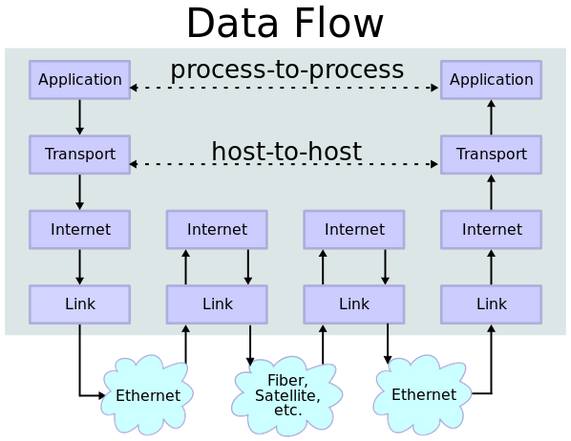
\includegraphics[scale=.5]{../pic/tcpip_model.png}
                \caption{Prikaz slojeva unutar TCP/IP modela komunikacije}
                \label{fig:tcpip_model}
        \end{figure}

        \subsection{Glavni principi arhitekture modela}

	Princip od kraja do kraja je evoluirao tokom vremena. Njegov prvobitni izraz je stavio
	odr\v{z}avanje stanja i sveobuhvatne inteligencije na ivice, i pretpostavio da internet koji je
	povezivao krajeve nije zadr\v{z}ao nikakvo stanje i koncentrisao se na brzinu i jednostavnost.
	Potrebe za za\v{s}titnim zidovima (\#\#[lazarc] firewalls \#\#), prevodiocima mre\v{z}nih adresa,
	ke\v{s}iranju sadr\v{z}aja sa interneta i sli\v{c}no, su izazvale promene u ovom principu.

	Princip robusnosti ka\v{z}e: "Uop\v{s}teno, implementacija mora biti konzervativna u pona\v{s}anju
	prilikom slanja i liberalna u svom pona\v{s}anju prilikom prijema. \v{S}to zna\v{c}i, da mora biti
	oprezna pri slanju dobro formiranih paketa (\#\#[lazarc] datagrams \#\#), ali mora
	prihvatiti bilo koji paket koji mo\v{z}e protuma\v{c}iti. (na primer, ne prime\'{c}ivati tehni\v{c}ke gre\v{s}ke
	gde nije poznato sta ih uzrokuje.)". "Drugi deo principa je gotovo jednako va\v{z}an: softver na
	drugim uredjajima mo\v{z}e sadr\v{z}ati razlike koji \v{c}ine nerazumnim da se iskoriste legalne, ali
	nejasne karakteristike protokola".

	Enkapsulacija se koristi za obezbedjivanje apstrakcije protokola i usluga. Enkapsulacija je
	obi\v{c}no uskladjena sa podelom unutar protokola na slojeve funkcionalnosti. Uop\v{s}teno,
	aplikacija (najvi\v{s}i nivo modela) koristi skup protokola za slanje svojih podataka kroz
	slojeve. Podaci se dalje enkapsuliraju na svakom sloju.

	Rani dokumenti o ovom protokolu, govore o \v{c}etvoroslojevnom protokolu. \v{S}to je u upotrebi i
	danas. I oni su unutar protokola kori\v{s}\'{c}eni u istom redosledu u kom \'{c}e i ovde biti navedeni.

	\begin{itemize}
		\item Aplikativni sloj (Application layer):
		Aplikativni sloj je opseg unutar kog aplikacije kreiraju korisni\v{c}ke podatke i prenose
		ove podatke drugim aplikacijama na istom ili drugom uredjaju (hostu). Aplikacije ili
		procesi, koriste usluge koje pru\v{z}aju donji slojevi, posebno transportni sloj koji
		obezbedjuje pouzdane ili nepouzdane veze ka drugim procesima. Komunikacione partnere
		karakteri\v{s}e arhitektura aplikacije, kao \v{s}to su model klijent-server i umre\v{z}avanje
		ravnopravnih korisnika. Ovo je sloj u kome su svi protokoli vi\v{s}eg nivoa, kao \v{s}to su SMTP,
		 FTP, SSH, HTTP, i td. Procesi se adresiraju preko portova koji u su\v{s}tini predstavljaju
		 usluge.
		\item Transportni sloj (Transport layer):
		Transportni sloj obavlja komunikacije izmedju doma\'{c}ina, ili doma\'{c}ina na istim ili
		razli\v{c}itim uredjajima (hostovima) i na lokalnoj mre\v{z}i ili udaljenim mre\v{z}ama razdvojenim
		od rutera. Ovaj sloj obezbedjuje kanal za komunikacione potrebe aplikacija. UDP je
		osnovni protokol transportnog sloja koji pru\v{z}a nepouzdanu uslugu sa paketima. Protokol
		za kontrolu prenosa (TCP) omogu\'{c}ava kontrolu protoka, uspostavljanje veze i pouzdan
		prenos podataka.
		\item Internet sloj (Internet layer):
		Internet sloj razmenjuje pakete preko mre\v{z}e. Ovaj sloj obezbedjuje uniforman mre\v{z}ni
		interfejs koji skriva stvarnu topologiju (raspored) osnovnih mre\v{z}nih veza. Zbog toga se
		naziva i slojem koji uspostavlja rad na mre\v{z}i. Zaista, ovaj sloj defini\v{s}e i uspostavlja
		internet. Ovaj sloj defini\v{s}e strukture adresiranja i usmeravanja koje se koriste za
		pakete TCP/IP protokola. Primarni protokol u ovom opsegu je Internet protokol, koji
		definise IP adrese. Njegova slede\'{c}a funkcija u usmeravanju je da prenosi pakete
		na slede\'{c}i IP ruter koji ima vezu sa mre\v{z}om bli\v{z}e kranjem odredi\v{s}tu podataka.
		\item Sloj veze (Link layer):
		Sloj veze defini\v{s}e metode umre\v{z}avanja u okviru lokalne mre\v{z}ne veze na kojoj uredjaji
		(hostovi) komuniciraju bez rutera u medjukomunikaciji. Ovaj sloj uklju\v{c}uje protokole
		koji se koriste za opisivanje topologije lokalne mre\v{z}e i potrebnih interfejsa da bi se
		zavr\v{s}io prenos paketa sa Internet sloja na ostale uredjaje.
	\end{itemize}

        \begin{figure}[htb]
                \centering
                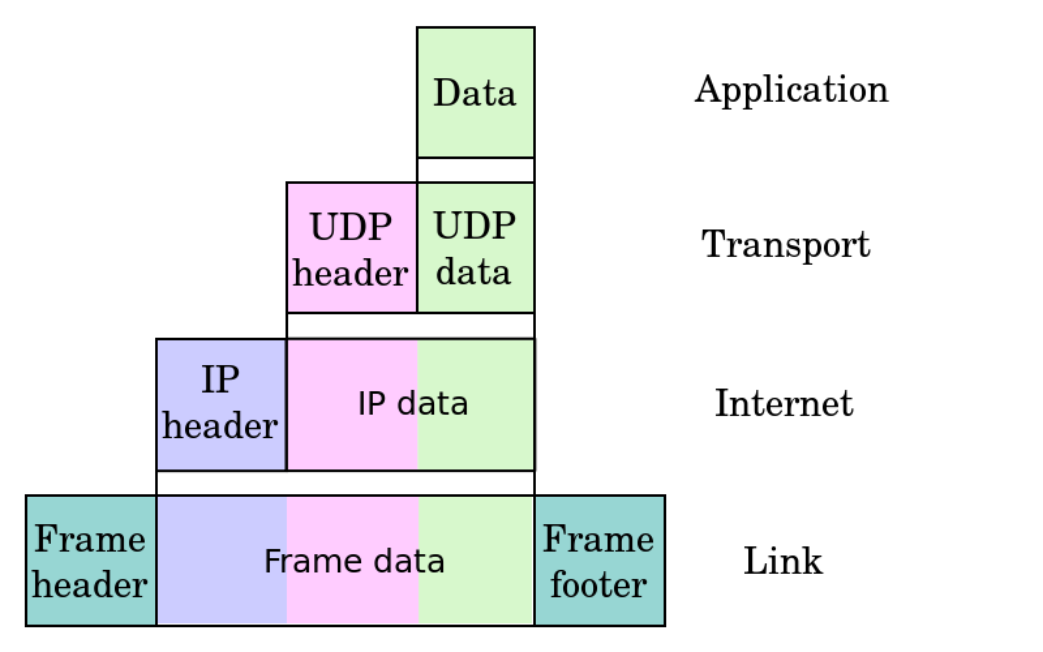
\includegraphics[scale=.4]{../pic/tcpip_data.png}
                \caption{Prikaz poruke koja se prenosi prema TCP/IP modelu komunikacije}
                \label{fig:tcpip_data}
        \end{figure}

        Slojevi protokola blizu vrha su logi\v{c}no bli\v{z}i korisnickoj aplikaciji, dok su oni bli\v{z}e dnu
	logi\v{c}ki bli\v{z}i fizi\v{c}kom prenosu podataka. Pregled slojeva u smislu pru\v{z}anja i kori\v{s}\'{c}enja
	usluge je metoda aplikacije koja izoluje gornje slojeve protokola od detalja kao \v{s}to je
	prenos bitova, detekcije lo\v{s}eg prenosa, na primer, dok su ni\v{z}i slojevi izolovani od detalja
	aplikacije i principa rada aplikacije.

	\section{Precission Time Protocol}

	Protokol preciznog vremena (Precision Time Protocol (PTP)) je protokol
	kori\v{s}\'{c}en za sinhronizaciju satova preko kompjuterske mre\v{z}e. U lokalnoj
	kompjuterskoj mre\v{z}i (local area connection), posti\v{z}e se preciznost sata i u rangu
	ispod mikrosekunde, \v{s}to ga \v{c}ini pogodnim za merenja i kontrolne sisteme.

	PTP je originalno definisan u IEEE 1588-2002 standardu, i zvani\v{c}no nazvan
	``Standard for a Precision Clock Synchronization Protocol for Networked Measurement
	and Control Systems'' i objavljen 2002 godine. U 2008 godini, IEEE 1588-2002 je
        objavljen kao preradjen standard, poznat i kao PTP Version 2, sa pobolj\v{s}anom
        ta\v{c}no\v{s}\'{c}u, precizno\v{s}\'{c}u i robusno\v{s}\'{c}u, medjutim nije kompatibilan
        sa prethodnom verzijom koja je objavljena 2002 godine.

	``IEEE 1588 je dizajniran da popuni prazninu koja nije dobro obradjena ni jednim od dva
	dominantna protokola, NTP i GPS\@. IEEE 1588 je dizajniran za lokalne sisteme u kojima je
	potrebna preciznost izvan one koja je dostupna NTP protokolom. Takodje je dizajniran za
	aplikacije koje se ne mogu nositi sa cenom GPS prijemnika na svakom uredjaju, ili sa onima
        u kojima nije mogu\'{c}e dobijanje GPS signala.'' (``IEEE 1588 is designed to fill a niche
        not well served by either of the two dominant protocols, NTP and GPS\@. IEEE 1588 is designed
        for local systems requiring accuracies beyond those attainable using NTP\@. It is also designed
        for applications that cannot bear the cost of a GPS receiver at each node, or for which GPS
        signals are inaccessible.'' - Eidson, John C. (April 2006). Measurement, Control and
        Communication Using IEEE 1588. Springer. ISBN 1-84628-250-0.

        \subsection{Arhitektura}

	IEEE 1588 standard opisuje hijerarhijsku master-slave arhitekturu za distribuciju vremena.
	Pod	ovom arhitekturom podrazumeva se distribucija vremena u sistemu koji se sastoji od
	jednog ili vi\v{s}e komunikacionih medijuma (segmenata koji su povezani na mre\v{z}u), i jednog
        ili vi\v{s}e izvora ta\v{c}nog vremena. \#Obi\v{c}ni uredjaj\# Izvor ``obi\v{c}nog'' vremena
        (``ordinary clock'') je uredjaj sa jednim pristupom mre\v{z}i i ima jednu od dve uloge, ili je
        izvor (master) ta\v{c}nog vremena, ili \v{c}eka na ta\v{c}no vreme (slave) u komunikaciji na
        mre\v{z}i. \#Sporedni uredjaj\# Grani\v{c}ni sat (Boundary	clock) ima vi\v{s}e pristupa, na
        razli\v{c}ite mre\v{z}e, i mo\v{z}e precizno sinhronizovati jedan segment mre\v{z}e na drugi.
        Master sinhronizacije se bira za svaki segment mre\v{z}e u sistemu. \#Glavni uredjaj\#
        Referentno vreme koje se uzima za izvor sinhronizacionog sata se zove Grandmaster clock.
        Grandmaster dostavlja sinhronizacione informacije do svih uredjaja koji su povezani na istu
        mre\v{z}u sa njim. Ukoliko se u nekom delu mre\v{z}e nalazi Boundary clock on prosledjuje
        ta\v{c}no vreme ka ostalim uredjajima koji su direktno na njega povezani.

        \begin{figure}[htb]
                \centering
                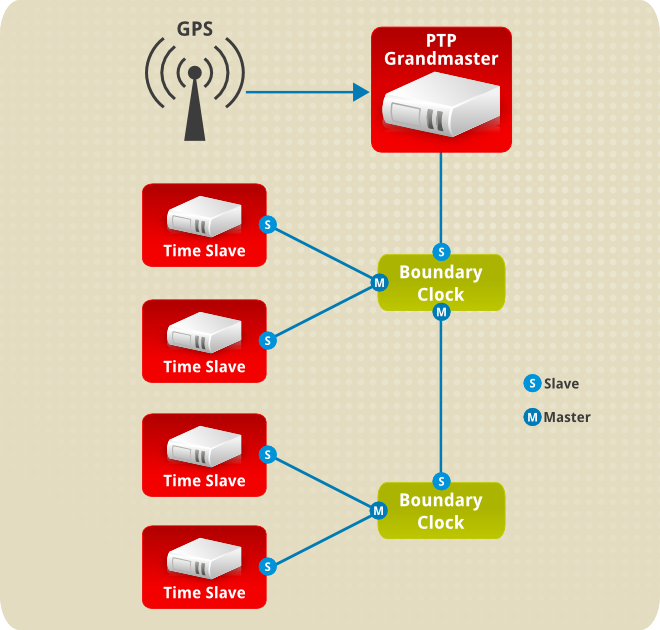
\includegraphics[scale=.3]{../pic/arch_ptp_system.png}
                \caption{Prikaz arhitekture jednog sistema koji podrzava PTP}
                \label{fig:arch_ptp_system}
        \end{figure}

	Simplifikovano, PTP sistem se sastoji od Ordinary clocks \#Obicnog uredjaja\# poveznih na
	jednostavnu mre\v{z}u, i bez Boundary clocks \#Sporednih uredjaja\#. Grandmaster se bira, i svi
	ostali uredjaji se direktno sinhroni\v{s}u na njega.

	IEEE 1588-2008 predstavljaju Clock koji je povezan sa mre\v{z}nom opremom koja prenosi PTP
	poruke.	Transparent clock \#Transparentni uredjaj\# modifikuje PTP poruke koje prolaze
	kroz uredjaj. Vremenski pe\v{c}ati (TIMESTAMPs) u porukama su modifikovani tako da se uzme u
	obzir i vreme za koje poruka prolazi kroz dodatne uredjaje u komunikaciji. Ova \v{s}ema
	komunikacije povecava distribuciju preciznosti tako \v{s}to se kompenzuje promenljivost
	dostave podataka preko mre\v{z}e.

	PTP tipi\v{c}no koristi EPOCH vreme, standardno vreme za UNIX sisteme (1 Januar 1970 kao
        po\v{c}etak ra\v{c}unanja vremena). Dok je UNIX vreme bazirano na Univerzalnom vremenu UTC,
        i mora da postoji sekunda preskoka (\#Ovo dodati, mozda u uvod\#), PTP je baziran na
	Medjunarodnom Atomskom Vremenu (TAI - International Atomic Time). PTP Grandmaster daje
	trenutnu razliku izmedju UTC i TAI, kako bi UTC vreme moglo da se izra\v{c}una od primljenog
	PTP vremena.

	\# mora slika da se vidi razlika izmedju UTC i PTP, TAI

        \subsection{Detalji protokola}

	Sinhronizacija i obrada u PTP sistemu se posti\v{z}e razmenom poruka preko komunikacionog
	medijuma. Do sad, PTP standard propisuje samo ove tipove poruka.

        \begin{itemize}
	    \item Sync, Follow\_Up, Delay\_Req i Delay\_Resp poruke se koriste u Ordinary i Boundary
	    uredjajima i slu\v{z}e samo za razmenu informacija o vremenu koje se koriste za
	    sinhronizaciju uredjaja na mre\v{z}i.
	    \item Pdelay\_Req, Pdelay\_Resp i Pdelay\_Res\_Follow\_Up se koriste u Transparent Clock
	    uredjajima da mere ka\v{s}njenje kroz uredjaj tako da se mo\v{z}e iskoristiti u kompenzaciji
	    vremena u sistemu. Transparent Clock i definicija ovih poruka nisu dostupne u IEEE
	    1588-2002 standardu.
	    \item Announce poruke se koriste i Best master clock algorithm u IEEE 1588-2002 standardu za
	    algoritam odredjivanja najta\v{c}nijeg sata na mre\v{z}i, i to kako bi se izgradila hijerarhija
	    uredjaja i kako bi se odredio Grandmaster.
            \item Management poruke se koriste u upravljanju mre\v{z}om za posmatranje performansi na
            mre\v{z}i, konfiguraciju mre\v{z}e i odr\v{z}avanje PTP sistema.
	    \item Signalne poruke se koriste u komunikaciji izmedju uredjaja koje nisu vremenski kriti\v{c}ne.
            Signalne poruke su uvedene u IEEE 1588-2002 standard.
        \end{itemize}

	Poruke se karakterizuju kao Event i General, odnosno poruke dogadjaja i opste poruke. Event
	poruke su vremenski kriti\v{c}ne i to u preciznosti predaje i prijema preciznosti vremenskih
	pe\v{c}ata (TIMESTAMPs) i direktno uti\v{c}u na distribuciju preciznosti vremena. (JOS JEDNOM
	POGLEDAJ OVAJ PREVOD). Sync, Delay\_Req, Pdelay\_Req i Pdelay\_resp su poruke dogadjaja.
	Op\v{s}te poruke su ubi\v{c}ajene jedinice protokola, zato \v{s}to su podaci u ovim porukama od
	zna\v{c}aja za PTP, ali njihovi vremenski pe\v{c}ati za predaju i prijem nisu. Announce, Follow\_Up,
	Delay\_Resp, Pdelay\_Resp\_Follow\_Up, Management i Signalne poruke su op\v{s}te poruke.

        \subsection{Prenos poruka}

	PTP poruke mogu da koriste UDP (User datagram portocol) preko Internet protokola (UDP/IP)
	za prenos poruka. IEEE 1588-2002, koristi samo IPv4 prenos, ali je ovo pro\v{s}ireno da
	uklju\v{c}uje i IPv6 u IEEE 1588-2008 standardu. U IEEE 1588-2002, sve PTP poruke se \v{s}alju u
	Multicast (modulu objavljivanja na mre\v{z}i) (\#pogldedaj opet ovaj prevod\#), dok je u IEEE
	1588-2008 to uvedeno kao opcija.

	\subsection{Algoritam najboljeg sata}
        BMC \(Best master clock algorithm\) algoritam obavlja deljenu selekciju najboljeg kandidata
        za ta\v{c}no vreme prema slede\'{c}im karakteristikama:

        \begin{itemize}
            \item Identifikator: Univerzalni jednistveni identifikator za sat. Tipi\v{c}no je baziran
            na MAC adresi uredjaja.
            \item Kvalitet: Obe verzije IEEE 1588 standarda poku\v{s}avaju da kvantifikuju kvalitet sata
            na osnovu o\v{c}ekivanih devijacija u vremenu, tehnologije koja je kori\v{s}\'{c}ena za
            implemntaciju vremena ili lokacije u hijerarhiji satova, u \v{s}emi kvaliteta satova
            (clock stratum scheme).
            \item Prioritet: Administrativno dodeljen prioritetni znak koji BMC koristi kako bi \v{s}to
            bolje odredio Grandmaster u PTP domenu. Dok je IEEE 1588-2002 standard imao samo jednu logi\v{c}ku
                promenljivu kako bi odredio prioritet, IEEE 1588-2008 ima dva 8-bitna polja prioriteta.
            \item Varijansa: Procena stabilnosti sata zasnovana na zapa\v{z}anju njegovog u\v{c}inka prema PTP
                refernci.
        \end{itemize}

	IEEE 1588 koristi hijerarhijski algoritam selekcije zasnovan na slede\'{c}im osobinama, u
	nazna\v{c}enom redosledu:

        \begin{itemize}
            \item Prioritet 1: korisnik mo\v{z}e dodeliti specifi\v{c}an stati\v{c}ki dizajniran prioritet
            svakom satu pre	svega odredjuju\'{c}i prioritet medju njima. Manje vrednosti prioriteta
            ozna\v{c}avaju ve\'{c}i prioritet.
                \item Klasa: Svaki sat je \v{c}lan odredjene klase, svaka klasa dobija svoj prioritet.
                \item Preciznost: Preciznost izmedju sata i UTC, u nanosekundama.
                \item Varijansa: Varijabilnost sata.
            \item Prioritet 2: Definisan prioritet, defini\v{s}u\'{c}i redosled rezervne kopije u slu\v{c}aju
            da drugi kriterijumi nisu dovoljni. Manje vrednosti prioriteta ozna\v{c}avaju ve\'{c}i prioritet.
                \item Jedinstveni identifikator: selekcija zasnovana na MAC adresi se koristi kao metod
                odlu\v{c}ivanja	kada su sve ostale osobine iste.
        \end{itemize}

        Svojstva sata se daju u IEEE 1588-2002 standardu porukama za sinhronizaciju (Sync messages) i u
        IEEE 1588-2008 standardu u porukama za ogla\v{s}avanje (Announce messages). Trenutni Master clock
	prenosi sve informacije u rednovnim intervalima. Sat koji sebe smatra boljim od trenutnog Master
        sata prenosi\'{c}e ove informacije kako bi se pozvali svi uredjaji za
        pormenu Master sata. Kada trenutni Master prepozna bolji sat, tada Master sat
	zaustavlja emitovanje poruka za sinhronizaciju (Sync Messages), ili poruke ogra\v{s}avanja
	(Announce messages), u zavisnosti od verzije protokola, i bolji sat preuzima ulogu Master
	sata. BMC algoritam uzima u obzir samo osobine koje su ve\'{c} poznate, i koje su deklarisali
	sami satovi, i ne uzima u obzir kvalitet veze na mre\v{z}i.

	\subsection{Sinhronizacija}

	Koriste\'{c}i BMC algoritam, PTP bira Master sat za IEEE 1588 domen i za svaki segment mre\v{z}e
        unutar tog domena. Satovi odredjuju razliku izmedju njih (offset) i Master-a na mre\v{z}i. Neka
        promenjiva $t$ predstavlja fizi\v{c}ki vreme. Za dati Slave uredjaj, razlika $o(t)$ u vremenu $t$
        se defini\v{s}e kao:

        \begin{equation}
            o(t) = s(t) - m(t)
        \end{equation}

	gde $s(t)$ predstavlja vreme mereno satom na Slave uredjaju u vremenu $t$, dok $m(t)$
	predstavlja vreme mereno satom na Master uredjaju u vremenu $t$.

	Master uredjaj periodi\v{c}no objavljuje (Broadcasts) trenutno vreme kao poruku ostalim
	uredjajima na mre\v{z}i. IEEE 1588-2002 protokolom je definisana objava vremena na svaku
	sekundu. Dok je IEEE 1588-2008 protokolom dozvoljeno i do 10 objava vremena u jednoj
	sekundi.

        \begin{figure}[htb]
                \centering
                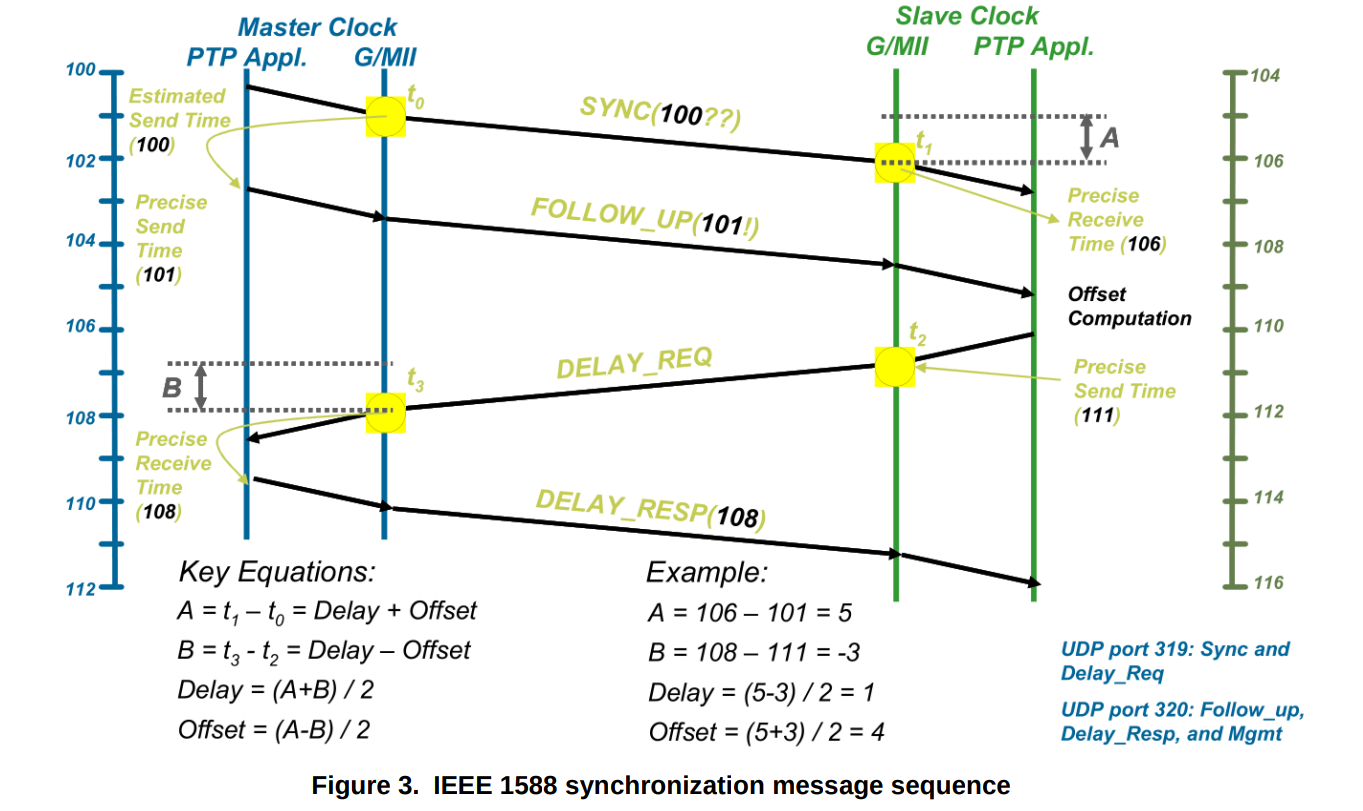
\includegraphics[scale=.3]{../pic/ieee_1588_sync_sequence.png}
                \caption{Prikaz sinhronizacione sekvence PTP protokola}
                \label{fig:ieee_1588_sync_sequence}
        \end{figure}

        Svaka objava vremena kre\'{c}e u vremenskom trenutku $T_1$, i to Sync porukom koju \v{s}alje
        Master uredjaj svim uredjajima u domenu. Uredjaj koji prima ovu poruku pamti vreme $T_1'$ u
        kom je primio Sync poruku. Master mo\v{z}e naknadno poslati Follow\_up poruku u kojoj \'{c}e
        se nalaziti ta\v{c}no vreme $T_1$ u kom je poslata prethodna poruka. Nemaju svi Master uredjaji
        sposobnost da po\v{s}alju ta\v{c}ne vremenske oznake unutar Sync poruke. Tek nakon \v{s}to je
        prenos zavr\v{s}en, oni mogu dobaviti ta\v{c}ne vremenske trenutke stizanja Sync poruke iz
        hardvera za povezivanje na mre\v{z}u. Master uredjaji sa ovim ograni\v{c}enjima \v{s}alju
        Follow\_up poruke kako bi preneli vreme $T_1$. Master uredjaji koji poseduju PTP mogu\'{c}nosti
        unutar hardvera za povezivanje mogu ubaciti ta\v{c}ne vremenske oznake unutar Sync poruka, i
        ne moraju koristiti Follow\_up poruke.

	Kako bi se ta\v{c}no sinhronizovali na Master uredjaj, satovi moraju individualno odrediti
	vreme prenosa poruka kroz medijum za povezivanje. Vreme progresije poruke kroz medijum za
	povezivanje	se radi merenjem vremena koje je potrebno da poruka ode od svakog uredjaja do
	njihovog Mastera u domenu, i da se vrati nazad. Ovu razmenu iniciraju Slave uredjaji i pri
        tome mere vreme progresije poruke $d$. Razmena poruka po\v{c}inje tako \v{s}to Slave uredjaj
        \v{s}alje Delay\_Req poruku u vremenskom trenutku $T_2$ ka svom Master uredjaju. Master uredjaj
	primi ovu poruku, i kao	odgovor po\v{s}alje ta\v{c}nu vremensku oznaku kada je primio Delay\_Req
	poruku. Poruka odgovora	Delay\_Resp sadrzi ta\v{c}no vreme $T_2'$ u kome je primljena poruka
	Delay\_Req.

	Nakon razmene ovih poruka Slave uredjaj ima spoznaju o \v{c}etiri vremenska trenutka $T_1$,
	$T_1'$,	$T_2$ i $T_2'$.

	Ukoliko je $d$ vreme koje je potrebno Sync poruci da prodje kroz medijum za povezivanje, a
        $\tilde{o}$ konstantna razlika satova izmedju Master i Slave uredjaja, onda je:

	\begin{equation}
		T_1' - T_1 = \tilde{o} + d
	\end{equation}

	i

	\begin{equation}
			T_2' - T_2 = -\tilde{o} + d
	\end{equation}

	Odakle je:

	\begin{equation}
		\tilde{o} = \frac{1}{2} (T_1' - T_1 - T_2' + T_2)
	\end{equation}

	Sada dva uredjaja znaju koliki je ofset $\tilde{o}$ prilikom prenosa i mogu se ispraviti
	tako da budu u skladu sa Master uredjajem.

	Jedna pretpostavka je da se prenos poruka odvija u periodu vremena koji je tako mali, da se
	razlika moze smatrati konstantnom u tom periodu. Jos jedna pretpostavka je da je vreme
	koje je	potrebno da poruka stigne od Master do Slave uredjaja ista kao i u obrnutom smeru.
	I na kraju, pretpostavka je da i Master i Slave uredjaji mogu da precizno mere vremenske
        trenutke u kojima \v{s}alju ili primaju poruke. Stepen primene ovih pretpostavki uti\v{c}e
        na to koliko \'{c}e se dobro sinhronizovati dva uredjaja.

        \#\# [lazarc] Pogledaj jos da se ubaci sa Teams za Valeo

	\newpage

	\chapter{Operativni sistem}

	\section{FreeRTOS}

	FreeRTOS je kernel operativnog sistema koji radi u realnom vremenu, i to za namenske
	sisteme, i mo\v{z}e se koristiti na velikom broju mikrokontrolera. FreeRTOS je idealno sklopljen
	za duboke namenske aplikacije u realnom vremenu koje koriste mikrokontrolere ili male mikroprocesore.
	Ovaj na\v{c}in projektovanja aplikacija uklju\v{c}uje kombinaciju kako strogih zahteva za realnim
	vremenom u aplikaciji, tako i manje strogih.

	Strogi zahtevi za aplikacijama realnog vremena su oni u kojima postoji vremenski rok u
	izvr\v{s}avanju, i ako se taj rok probije, do\'{c}i ce do apsolutnog pada funkcionalnosti sistema.
	Na primer, airbag u kolima ima potencijal da napravi vi\v{s}e \v{s}tete nego dobrog ukoliko je
	odziv sistema samo malo sporiji nego \v{s}to treba.

	FreeRTOS je kernel realnog vrmena (ili rasporedjiva\v{c} realnog
	vremena) na	koji se nadogradjuje aplikacija tako da ispuni stroge zahteve za realnim
	vremenom aplikacije. To dozvoljava da aplikacija bude organizovana kao kolekcija
	nezavisnih programskih niti. Na	procesoru koji ima samo jedno jezgro, samo jedna
	programska nit se mo\v{z}e izvr\v{s}avati u jednom trenutku. Kernel odlu\v{c}uje koja nit se
	izvr\v{s}ava tako \v{s}to odredjuje prioritet koji se dodeljuje svakoj niti. U najjednostavnijem
	slu\v{c}aju, dizajner aplikacije mo\v{z}e odrediti vi\v{s}e prioritete nitima koje implementiraju stroge
	zahteve za realnim vremenom, a ni\v{z}e prioritete onim nitima koje nemaju tako stroge zahteve
	za izvr\v{s}avanjem. Ovim bi se osiguralo da niti koje imaju stro\v{z}ije zahteve, imaju
	prioritete izvr\v{s}avanja i pristupa resursima nad ostalim nitima, ali odluke za dodelu
	izvr\v{s}avanja nisu uvek tako jednostavne.

	Napomena: Unutar FreeRTOS-a se programska nit naziva ``task''. Tako da \'{c}e se u daljem tekstu
	i koristiti naziv Task za programsku nit.

	U projektovanju aplikacija za namenske sistema postoji ustaljena praksa projektovanja
	aplikacija koja ne zahteva kori\v{s}\'{c}enje kernela za realno vreme, i ove tehnike mogu dati
	bolje re\v{s}enje problema. Mada, u kompleksnijim slu\v{c}ajevima, verovatnije je kori\v{s}\'{c}enje
	kernela za aplikacije u realnom vremenu, i takodje mo\v{z}e biti kombinacija kori\v{s}\'{c}enja
	kernela, i drugih tehnika projektovanja aplikacije.

	Kao \v{s}to je ve\'{c} opisano, prioriteti taskova mogu pomo\'{c}i da se osigura da aplikacija ispuni
	sve zahteve, ali kernel mo\v{z}e doneti i neke manje o\v{c}igledne beneficije. Neke od njih su
	navedene ispod:

	\begin{itemize}
		\item Skra\'{c}ivanje informacija o vremenskom rasporedu (Abstracting away timing information):
		Kernel je odgovoran za vreme izvr\v{s}avanja i dodeljuje API kojim se
		unutar aplikacije mo\v{z}e upravljati vremenom. Ovim se omogu\'{c}ava jednostavnija
		strukturiranost koda, i ukupna veli\v{c}ina koda je manja.
		\item Odr\v{z}avanje/Pro\v{s}irivanje (Maintainability/Extensibility):
		Uskra\'{c}ivanjem informacija o vremenskom rasporedu rezultuje u manjim zavisnostima
		izmedju	modula, i dozvoljava aplikaciji da evoluira na kontrolisan i predvidjen
		na\v{c}in. Takodje, kernel je odgovoran za rasporedjivanje vremena, tako da performanse
		aplikacije manje mogu biti promenjene u hardveru na kome se pokre\'{c}u.
		\item Modularnost (Modularity):
		Taskovi su nezavisni moduli, pri \v{c}emu svaki od njih mora imati dobro definisanu svrhu.
		\item Timski razvoj (Team development):
		Taskovi bi trebalo da imaju dobro definisane interfejse, kako bi se lak\v{s}e razvijali u
		timovima.
		\item Lak\v{s}e testiranje (Easier testing):
		Ako su takskovi dobro definisani kao nezavisni moduli sa \v{c}istim interfejsima, mogu biti
		testirani nezavnisno.
		\item Ponovno kori\v{s}\'{c}enje koda (Code reuse):
		Ve\'{c}a modularnost sa ve\'{c}om nezavisno\v{s}\'{c}u koda koji se mo\v{z}e ponovo koristiti
		sa manje ulo\v{z}enog truda.
		\item Pobolj\v{s}ana efikasnost (Improved efficiency):
		Kori\v{s}\'{c}enjem kernela softver se u popunosti mo\v{z}e prebaciti na pokretanje dogadjajima
		(event driven programming), i time bi se u\v{s}tedelo procesorsko vreme koje se tro\v{s}i na
		poliranje dogadjaja koji se ne dogadjaju. Kod se pokrece samo ukoliko postoji ne\v{s}to
		sto je potrebno	uraditi. Protiv pobolj\v{s}ane efikasnosti stoji to da je potrebno pocesuirati
		RTOS prekid, i promeniti izvr\v{s}avanje sa jednog taska na drugi. Kako god, i aplikacije koje ne
		koriste RTOS normalno uklju\v{c}uju neku formu prekida.
		\item Idle time:
		Idle task je task koji se automatski kreira prilikom startovanja Scheduler-a. I izvr\v{s}ava se
		kad nema taskova unutar aplikacije koji bi se izvr\v{s}avali. Ovaj task se mo\v{z}e koristiti za
		merenje procesorske mo\'{c}i koja se tro\v{s}i, za izvr\v{s}avanje provera u pozadini, ili da
		jednostavno pokrene re\v{z}im smanjene potro\v{s}nje u sistemu.
		\item Upravljanje snagom (Power management):
		Efikasnost koja se dobija kori\v{s}\'{c}enjem RTOS-a dozovoljava procesoru da provede vi\v{s}e
		vremena	u re\v{z}imu smanjene potro\v{s}nje. Potro\v{s}nja se mo\v{z}e zna\v{c}ajno smanjiti time
		\v{s}to procesor odlazi u re\v{z}im smanjenje potro\v{s}nje kad god je pokrenut Idle task. FreeRTOS
		takodje ima i specijalni tick-less mod, u kome procesor odlazi u re\v{z}im smanjene
		potro\v{s}nje na du\v{z}e vreme.
		\item Fleksibilno upravljanje prekidima (Flexible interrupt handling):
		Upravljanje prekidima se mo\v{z}e dr\v{z}ati veoma kratko tako \v{s}to se odla\v{z}e obrada bilo kog
		taska koji je kreirao sam dizajner, ili taska unutar FreeRTOS-a.
		\item Razli\v{c}iti zahtevi za obradom (Mixed processing requirements):
		Jednostavni oblici dizajniranja programa mogu se posti\'{c}i me\v{s}anjem periodi\v{c}nog,
		kontinualnog i procesiranja pokretanog dogadjajima. Pored toga, ispunjavanje strogih i
		manje strogih zahteva za realnim vremenom u aplikacijama mo\v{z}e se posti\'{c}i izborom
		odgovoaraju\'{c}ih taskova i prioriteta prekida.

	\end{itemize}

	\subsection{Implementacija}

	FreeRTOS je dizajniran tako da bude mali i jednostavan. Kernel (srce operativnog sistema)
	se sastoji od samo 3 fajla, i pisan je u C programskom jeziku. Kako bi se kod napravio da
	bude citljiv, lako portabilan, i kako bi se lako odr\v{z}avao projekat, pisan je uglavnom u C
	programskom jeziku, sa izuzetkom nekih funkcionalnosti koje su napisane u asembleru, gde je to
	bilo potrebno, i to uglavnom rutine u Scheduler-u (Rasporedjivacu niti) koje su specifi\v{c}ne
	za samu arhitekturu.

	FreeRTOS omogu\'{c}ava kori\v{s}\'{c}enje metoda za stvaranje vi\v{s}e programskih niti,
	ili Taskova, stvaranje mehanizama za Sinhronizaciju niti, Mutexa, Semafora i softverskih tajmera.
	Takodje, postoje mogu\'{c}nosti kori\v{s}\'{c}enja FreeRTOS-a i za aplikacije niske potro\v{s}nje.
	Aplikacije koje koriste FreeRTOS mogu biti kompletno stati\v{c}ki alocirane. Alternativno
	RTOS objekti mogu biti dinami\v{c}ki alocirani sa 5 \v{s}ema alokacije memorije i one su rasporedjene
	tako da pru\v{z}aju slede\'{c}e mogu\'{c}nosti:

	\begin{itemize}
		\item samo alociranje;
		\item alociranje i oslobodjanje sa jednostavnim, brzim algoritmom;
		\item kompleksnije ali br\v{z}e alokaciranje i oslobadjanje uz algoritam spajanja susednih
		memorijskih blokova;
		\item alternativa za jo\v{s} kompleksniju \v{s}emu koja uklju\v{c}uje spajanje susednih
		memorijskih	blokova	koja omogu\'{c}ava da hip (HEAP) bude podeljen na vi\v{s}e memorijskih
		delova;
		\item i na kraju C biblioteka za alociranje i oslobadjanje sa za\v{s}titom medjusobnog
		isklju\v{c}ivanja.
	\end{itemize}

	Unutar FreeRTOS-a ne postoji ni jedan od slo\v{z}enijih svojstava operativnih sistema koji se
	uobi\v{c}ajeno mogu na\'{c}i u operativnim sistemima poput Linux-a ili Microsoft Windows-a, kao
	\v{s}to su drajveri uredjaja, napredno upravljanje memorijom, korisni\v{c}ki nalozi, i
	umre\v{z}avanje. Akcenat ovog operativnog sistema je na kompaktnosti i brzini izvr\v{s}avanja. O
	FreeRTOS-u se mo\v{z}e misliti kao o "biblioteci niti" vise nego kao o "operativnom sistemu".

	FreeRTOS implementira vi\v{s}e niti tako \v{s}to postoji jedan program koji poziva metode niti u
	jednakim kratkim vremenskim intervalima. Metoda promene niti zavisi od prioriteta niti i
	uklju\v{c}uje round-robin \v{s}emu promene niti. Uobi\v{c}ajen interval promene je do $1/1000$ sekunde
	do $1/100$ sekunde, i to kroz prekid hardverskog tajmera, ali interval promene se \v{c}esto menja
	tako da zadovolji potrebe specifi\v{c}ne aplikacije.

	\section{lwIP}

	lwIP (light-weight IP) je implementacija TCP/IP komplet-a (\#\# [lazarc] [prevod] suite
	\#\#) je originalno napisao Adam Dunkels u Computer and Networks Architectures (CNA)
	laboratoriji na	\v{S}vedskom institutu za kompjuterske nauke (Swedish Institute of Computer
	Science) ali ga sad	aktivno razvija tim in\v{z}enjera \v{s}irom sveta kojim rukovodi Kieran
	Mansley\@.

	lwIP je open-source projekat koji je besplatan za preuzimanje i kori\v{s}\'{c}enje (pod BSD
	licencom), pisan u C programskom jeziku i mo\v{z}e se preuzeti sa internet stranice tima koji
	ga razvija.

	Fokus lwIP implementacije TCP/IP je da se smanji kori\v{s}\'{c}enje RAM memorije i da se i dalje
	dobija potpuna funcionalnost TCP\@. Ovim lwIP postaje interesantan za kori\v{s}\'{c}enje u namenskim
	sistemima koji raspola\v{z}u sa RAM memorijom od nekoliko desetina kilobajta (kB) i prostorom od
	oko 40kB u ROM memoriji.

	Od kada je prvi put objavljen, lwIP izaziva dosta interesovanja, i danas se koristi u dosta
	komercijalnih projekata\@. lwIP je do sad iskori\v{s}\'{c}en na mnogim platformama i operativnim
	sistemima, i mo\v{z}e se koristiti bez i sa operativnim sistemom. U ovoj implementaciji, lwIP
	se koristi u okviru FreeRTOS operativnog sistema, kao jedan njegov deo.

	LwIP je veoma modularan i ima podr\v{s}ku za dosta protokola, od kojih ve\'{c}ina mo\v{z}e da se
	ukloni za manju veli\v{c}inu koda.
	\begin{itemize}
		\item \textit{Mre\v{z}ni protokoli i protokoli veze: (Link and network protocols)}
		\begin{itemize}
			\item \textbf{ARP}: protokol veze koji se koristi za prevod prirodne hardver adrese
			("MAC adresa") u IP adresu
			\item \textbf{IPv4}: dominantni mre\v{z}ni protkol koji se koristi danas, posebno za
			Internet
			\item \textbf{IPv6}: naslednik IPv4, koji, naro\v{c}ito, pro\v{s}iruje veli\v{c}inu IP adrese
			na 128 bita
			\item \textbf{ICMP}: kontrolni protokol za IP
			\item \textbf{IGMP}: protokol za urpravljanje grupa unutar IP-a
		\end{itemize}
		\item \textit{Transportni protokoli: (Transport protocols)}
			\begin{itemize}
				\item \textbf{UDP}: protokol bez priklju\v{c}ka, i bez mehanizma pouzdanosti
				\item \textbf{TCP}: protokol orjentisan ka konekciji, za kontinualni tok
				podataka ("streaming")
			\end{itemize}
		\item \textit{Protokoli visokog nivoa: (High-level protocols)}
			\begin{itemize}
				\item \textbf{DHCP}: dobijanje IP adrese sa podr\v{s}kom servera
				\item \textbf{AUTOIP}: dobijanje IP adrese bez podr\v{s}ke servera
				\item \textbf{SNMP}: kori\v{s}\'{c}en za nadgledanje stanja mre\v{z}e
				\item \textbf{PPP}: kori\v{s}\'{c}en za stvaranje direktne konekcije izmedju dva \v{c}vora
				na mre\v{z}i
			\end{itemize}
	\end{itemize}

	IPv4: (\#\#[lazarc] opisati u delu za softversku implementaciju \#\#)

	lwIP pru\v{z}a tri API-a (Application Program's Interface) za programe koji komuniciraju sa
	TCP/IP kodom:
	\begin{itemize}
		\item low-level "core"/"callback" ili "raw" API
		\item dva API-a vi\v{s}eg nivoa (sekvencijalni API-i):
			\begin{itemize}
				\item netconn API
				\item socket API
			\end{itemize}
	\end{itemize}

	Sekvencijalni API pru\v{z}a na\v{c}in za obi\v{c}no, sekvencijalno programiranje koje koristi lwIP stek
	(stack). Model izvr\v{s}avanja je baziran na blokiraju\'{c}oj
	otvori-pro\v{c}itaj-upi\v{s}i-zatvori paradigmi. Kako je TCP/IP stek baziran na dogadjajima,
	TCP/IP kod i aplikativni program, moraju da se pozivaju sa razli\v{c}itim kontekstima
	izvr\v{s}avanja, u razli\v{c}itim nitima.

	Prilikom me\v{s}anja sekvencijalnog i "sirovog" API-a u programima, treba biti pa\v{z}ljiv.
	Funkcije koje pripadaju nesekvencijalnom API-u u stvari mogu biti pozvane iz glavne
	tcpip\_thread niti.
	Takodje, registrovanje programski rutina (ili inicijalizovanje delova u lwIP) mora biti
	odradjeno unutar tog konteksta (na primer, u vreme startovanja aplikacije u
	tcpip\_init\_callback rutini ili u vreme izvr\v{s}avanja unutar tcpip\_callback rutine).

	Jo\v{s} neke \v{c}injenice o API-ima koje uti\v{c}u na kori\v{s}\'{c}enje lwIP steka:
	\begin{itemize}
		\item \textbf{netconn- i raw-API su samo unutar lwIP-a :} kod koji koristi ovaj API se
		ne mo\v{z}e koristiti u drugim stekovima koji imaju iste mogu\'{c}nosti kao lwIP (na primer
		uIP i td.)
		\item \textbf{socket API} je u suprotnosti sa gore navedenom stavkom, napravljen je
		tako da je kompatibilan i mo\v{z}e se koristiti u drugim stekovima.
		\item \textbf{socket- i netconn-API} su sekvencijalni API-i koji zahtevaju programske
		niti (jedna nit je za aplikaciju koja koristi API, jedna nit upravlja tajmerima unutar
		steka, paketima koji dolaze, i td.)
		\item \textbf{raw API} koristi mehanizam povratnih rutina (na primer\@. aplikacija poziva
		rutinu kada dodje novi podatak). Ukoliko se koristi u programu koji radi na
		sekvencijalni na\v{c}in, mo\v{z}e biti te\v{z}e kori\v{s}\'{c}enje.
		\item \textbf{raw API} daje bolje performanse kako ne zahteva promenu izvr\v{s}avanja
		programskih niti.
		\item \textbf{raw API i netconn API} podr\v{z}avaju zero-copy \footnotemark{predstavlja
		operaciju pri kojoj procesor ne vr\v{s}i kopiranje podataka iz jedne memorijske oblasti u
		drugu. Ovo se \v{c}esto koristi kako bi se sa\v{c}uvali ciklusi procesora i propusnog opsega
		memorije prilikom prenosa kontinualnih podataka (datoteka, fajlova) preko mre\v{z}e.} kako
		za TX tako i za RX, tj\@. kako za predaju, tako i za prijem podataka.
	\end{itemize}

	\newpage

	\chapter{Hardverska implementacija}

	Razvojno okru\v{z}enje koje je kori\v{s}\'{c}eno za hardversku implementaciju je razvojna
	plo\v{c}a SAMA5D27-SOM1-EK1 proizvodja\v{c}a Microchip. Na plo\v{c}i se nalazi SAMA5D27
	SOM (System on Module) modul koji je klju\v{c}an za implementaciju. Na modulu se nalazi
	SAMA5D27-D1G-CU SIP (System in Package) koji sadr\v{z}i 1 Gbit DDR2 SDRAM memorije. Modul
	nudi puzdanu i niskobud\v{z}etnu platformu	za razvoj namenskih ra\v{c}unarskih sistema
	koji ce na kraju i zavr\v{s}iti u finalnoj proizvodnji, kao i malu formu, dopunjenu sa
	velikim brojem interfejsa koji se mogu koristiti u delu projektovanja krajnjeg sistema.

        \begin{figure}[htb]
                \centering
                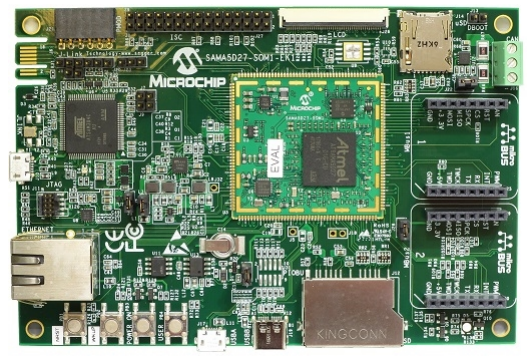
\includegraphics[scale=.7]{../pic/hw_top_view.png}
                \caption{Razvojna plo\v{c}a SAMA5D27-SOM1-EK1 (pogled odozgo)}
                \label{fig:hw_top_view}
        \end{figure}

	SOM je potpuno opremljen industrijski sertifikovan kompjuter dizajniran za integraciju
	korisni\v{c}ke aplikacije. SOM modul je namenski napravljen kao mala hardverska platforma
	opremljena \v{s}irokim spektrom modula za brzo povezivanje kako bi podr\v{z}ali
	projektovanje podr\v{s}ke za razne IoT (Internet of Things) aplikacije, prenosnih uredjaja,
	ali i aplikacija u industrijske svrhe. SOM integri\v{s}e 1Gbit DDR2 SDRAM i QSPI memoriju
	kao 10/100 Mbit Ethernet interfejs. Takodje, SOM poseduje i 128 GPIO pinova
	koji obezbedjuju pristup SOM-a za razli\v{c}ite upotrebe. Svi GPIO pinovi su nezavisni, i
	mogu se konfigurisati kao ulazi	ili izlazi, sa ili bez PULL-UP otpornika. Razvojna plo\v{c}a
	poseduje  i \v{s}irok spektar periferija, kao i korisni\v{c}ki interfejs i na\v{c}in za
	pro\v{s}irenje funkcionalnosti, uklju\v{c}uju\'{c}i i dva microBUS Click interfejsa firme
	Mikroelektronika kojim se dobija mogu\'{c}nost za pro\v{s}irenje funkcionalnosti svim
	modulima koje ova firma nudi u svom asortimanu.

        \begin{figure}[htb]
                \centering
                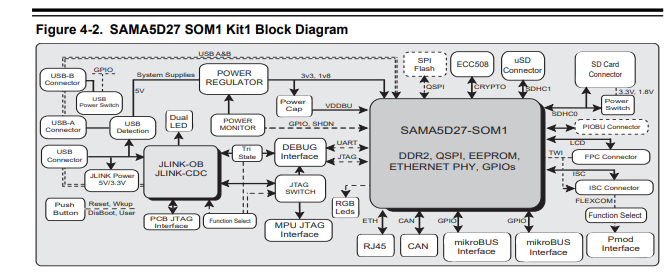
\includegraphics[scale=.7]{../pic/hw_modules.png}
                \caption{Moduli - Razvojna plo\v{c}a SAMA5D27-SOM1-EK1}
                \label{fig:hw_modules}
        \end{figure}

	Na samom SAMA5D27-SOM1 postoje i:
	\begin{itemize}
		\item Ultra mali SIP (SAMA5D27-D1G-CU) koji sadr\v{z}i \v{s}tedljivi SAMA5D27 Arm Cortex
		A5 procesor i 1Gbit DDR2 SDRAM memoriju
		\item SST26VF064 64 Mb QSPI Flash memoriju
		\item 24AA02E48 2 Kb serijski E2PROM (Electrically Erased Programmed Read Only Memory)
		sa programiranom EUI identifikacijom pristupa
		\item MIC2800 cip za kontrolu napajanja
		\item KSZ8081RNA Ethernet Phy 10/100 MHz RMII
	\end{itemize}

        \begin{figure}[htb]
                \centering
                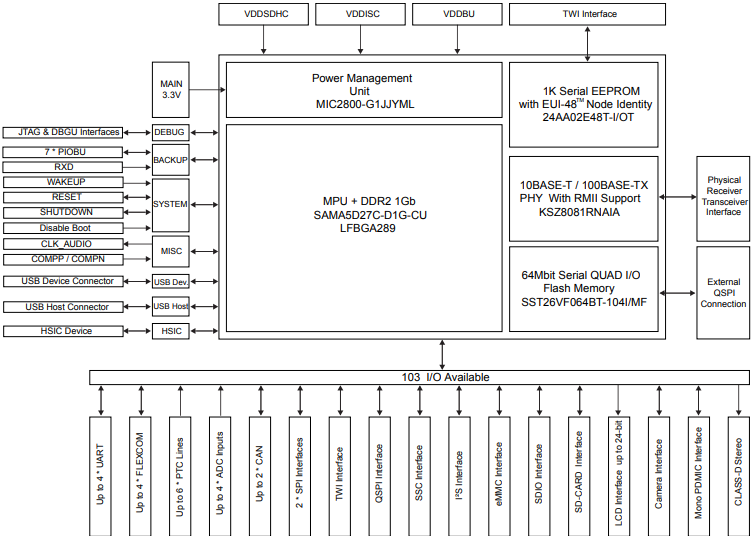
\includegraphics[scale=.5]{../pic/hw_som_modules.PNG}
                \caption{Moduli - SAMA5D27-SOM1}
                \label{fig:hw_som_modules}
        \end{figure}

	Razvojno okru\v{z}enje SAMA5D27-SOM1-EK1 je veoma mo\'{c}no i mo\v{z}e se koristiti za \v{s}
	irok spektar aplikacija. Naj\v{c}e\v{s}\'{c}e je izbor za razvoj aplikativnog softvera u
	namenskim ra\v{c}unarskim sistemima, uz kori\v{s}\'{c}enje Embedded Linux operativnog
	sistema, i s tim ciljem se i bira. Za ovu implementaciju nije kori\v{s}\'{c}en u tom smislu,
	ve\'{c} je kori\v{s}\'{c}en sa drugim operativnim sistemom kojim je mogu\'{c}e ista\'{c}i
	neke druge njegove karakteristike. Ali ono sto je najvi\v{s}e interesantno za ovu primenu je
	postojanje TSU (Timestamping unit) za harversku podr\v{s}ku PTP-a. I to u sklopu periferije
        za povezivanje preko Ethernet-a, \v{c}ime je omogu\'{c}eno prepoznavanje PTP poruka koje dolaze
	na interfejs.

	\section{Timestamping unit - TSU}
        Timestamping unit (TSU), je periferija unutar procesora koja pru\v{z}a
        podr\v{s}ku prilikom vremenskog ozna\v{c}avanja paketa koji
        u\v{c}estvuju u razmeni poruka u PTP protokolu. TSU se sastoji od
        tajmera, koji je implementiran kao broja\v{c}, i registara u koji se
        sme\v{s}taju vremena u kojima PTP paketi prelaze granicu vremenskog
        ozna\v{c}avanja. Hardverski prekid se registruje prilikom
        osve\v{z}avanja registara, pri \v{c}emu se osve\v{z}avanje registara
        dogadja svaki put kada ta\v{c}no specificirani paketi predju preko
        interfejsa.

        Tajmer unutar periferije je implementiran kao 94 bitni broja\v{c}, kod
        koga je najvi\v{s}ih bita predstavlja broj sekundi, slede\'{c}ih 30
        bita predstavlja broj nanosekundi i najni\v{z}ih 16 bita predstavlja
        vreme nivoa ispod nanosekunde. Donjih 46 bita se prebroje nakon \v{s}to
        je izbrojena jedna sekunda, i takodje prijavljuje se prekid kada se
        izbroji jedna sekunda. Vrednost tajmera je mogu\'{c}e pro\v{c}itati,
        kao i modifikovati preko APB interfejsa. Frekvencija tajmera se dobija
        od MCK procesora. U ovom slu\v{c}aju MCK je 82MHz.

        Veli\v{c}ina inkrementa tajmera je podesiva i mo\v{z}e se kontrolisati
        preko registra GMAC\_TI, gde je donjih 8 bita vrednost za koju \'{c}e
        se uve\'{c}ati vrednost tajmera u nanosekundama, i dodatnih 16 bita
        unutar registra GMAC\_TISUBN, unutar koga se specificira vrednost
        inkrementa na nivou vremena ispod nanosekunde. Ukoliko je ostatak
        registra GMAC\_TI nula, na svaku uzlaznu ivicu kloka koji dolazi na
        periferiju, vrednost \'{c}e se uve\'{c}avati za vrednost donjih 8 bita
        GMAC\_TI registra, plus vrednost GMAC\_TISUBN registra. Registar
        GMAC\_TISUBN dozvoljava rezoluciju od otprilike 15 femtosekundi.

        Takodje, registar GMAC\_TI ima mogu\'{c}nost pode\v{s}avanja
        alternativnog broja nanosekundi, i to na bitima od 15 do 8, i na bitima
        od 23 do 16 broj ciklusa nakon koga \'{c}e se iskoristiti vrednost
        alternativnog broja nanosekundi prilikom uve\'{c}anja vrednosti
        broja\v{c}a. Ovaj deo periferije je u velikoj meri zna\v{c}ajan za
        pode\v{s}avanje ta\v{c}nog vremena, i to u slu\v{c}ajevima kada se
        koriste drugi oscilatori za pogon procesora, koji daju druga\v{c}ije
        vrednosti frekvencije kojom se uve\'{c}ava vrednost broja\v{c}a.

        Ova periferija najvi\v{s}e uti\v{c}e na ta\v{c}no vreme koje je potrebno
        sinhronizovati, i takodje daje informacije o ta\v{c}nom vremenu na uredjaju
        koji se koristi. Vi\v{s}e detalja o samoj implemntaciji i kori\v{s}\'{c}enju
        ove periferije bi\'{c}e dato u delu softverske implementacije.

	\newpage

	\chapter{Softverska implementacija}

        U ovom delu \'{c}e biti opisana softverska implementacija projekta, sa
        datim rezultatima na kraju odeljka. Rezultati se odnose na razliku u
        satovima dva uredjaja u sistemu koji je napravljen kako bi se prikazala
        funkcionalnost protkola, i izvr\v{s}ila sinhronizacija dva uredjaja
        unutar oglednog sistema.

        \#\# Prikaz sistema, nparaviti sliku gde se vide Linux PC i ploca

        Ogledni sistem za implementaciju protokola preciznog vremena se sastoji
        od PC-a, na kome se nalazi Ubuntu 16.04 LTS operativni sistem, i
        razvojne plo\v{c}e SAMA5D27-SOM1-EK1. Povezivanje izmedju razvojne
        plo\v{c}e i PC-a je ostvareno preko standardnog UTP kabla (UTP -
        Unshielded-Twisted-Pair). Na PC-u se pokre\'{c}e Open source
        implementacija PTPd, odnosno deamon-a koji obavlja funkciju PTP
        protokola na standardnim operativnim sistemima. U ovom slu\v{c}aju je
        izabran PTPd kao najjednostavnija i najdostupnija verzija ovakvog
        programa koja se pravljena za operativne sisteme bazirane na Linux-u.

        Kako je u nekim trenucima potrebno da vi\v{s}e uredjaja na mre\v{z}i
        dobija informacije potrebne za sinhronizaciju, sam PTP deamon je
        konfigurisan da radi u Master only modu, i takodje u Multicast modu.
        \v{S}to zna\v{c}i da je Linux PC u ovoj konfiguraciji oglednog sistema
        uvek Master i da svi uredjaji moraju da se sinhroni\v{s}u na njegovo
        ta\v{c}no vreme. Takodje, kako je PC jedini uredjaj na mre\v{z}i koji
        daje takve informacije, postavljen je u Mulitcast mod, tako da svi
        uredjaji dobijaju informacije, dok samo neki koji mogu da prepoznaju
        odredjene poruke, mogu da odgovore i sinhroni\v{s}u se u potpunosti. S
        tim u vezi, dodata su jos neka pode\v{s}avanja samog deamon-a, \v{c}ime
        je odredjen period za odgovor sa slave strane, odnosno da ukoliko ne
        dodje do odgovora u nekom roku, PC nastavi da \v{s}alje generi\v{c}ke
        poruke, kako bi pokrenuo proces sinhronizacije. Takodje, u svrhe
        provere da li je sve pode\v{s}eno na najbolji na\v{c}in, vr\v{s}i se
        pra\'{c}enje svih poruka koje se dobijaju i skladi\v{s}te na PC-u kako
        bi kasnije mogle da se provere, ukoliko dolazi do gre\v{s}aka na
        mre\v{z}i. Kako se koristi PC, odnosno kompjuter op\v{s}te namene, koji
        je preko jednog od interfejsa, povezan na internet, sam PC dobija
        ta\v{c}no vreme preko NTP-a, nakon \v{c}ega to vreme postaje najbolje
        za lokalnu oglednu mre\v{z}u. Ukoliko bi se koristio specijalizovani
        kompjuter, koji ima mogu\'{c}nost da ta\v{c}no vreme dobije preko
        GPS-a, i takodje specijalizovane mre\v{z}ne kartice, koje
        podr\v{z}avaju PTP, mogla bi se dobiti mnogo ve\'{c}a ta\v{c}nost, i
        time bi se pove\'{c}ala ta\v{c}nost na slave uredjaju koji poku\v{s}ava
        da se sinhroni\v{s}e. Implementacija PTP deamon-a na PC-u je preuzeta i
        kori\v{s}\'{c}ena u skladu sa uslovima i preporukama Open Source
        zajednice, i sem konfiguracije ni\v{s}ta nije promenjeno, kako bi se
        prilagodilo ovoj implementaciji.

        Sa druge strane, implementacija na slave strani, u ovom slu\v{c}aju na
        evaluacionoj plo\v{c}i, je morala biti prilagodjena samom PTP
        protokolu, i morala je obezbediti mehanizme za korektno kori\v{s}\'{c}enje
        PTP protokola.

        Softverska implementacija je zami\v{s}ljena tako da se mo\v{z}e
        obezbediti lako dodavanje novih funkcionalnosti, kao i promena ve\'{c}
        postoje\'{c}ih funckionalnosti u vrlo kratkom vremenskom roku. S tim u
        vezi izabran je FreeRTOS kao operativni sistem koji ce biti osnova, i
        odabrana je Multi-Threaded arhitektura softvera koji implementira ovu
        funkcionalnost. Odabir ovog operativnog sistema i ove arhitekture je
        usko vezan sa svim \v{s}to je potrebno iskoristiti kako bi se
        obezbedila korektna implementacija ovog protokola. Kao i dostupnost
        baze znanja za ovaj operativni sistem, i njegova Open Source priroda.
        Takodje, za IP stack je izabran lwIP stack, koji je pogodan za
        implementacije na Embedded uredjajima, i takodje je Open Source i ima
        \v{s}iroko dostupnu bazu znanja.

        Implementacija ostavlja mogu\'{c}nosti za dodavanje novih
        funkcionalnosti, i to kao dodavanje novih thread-ova
        unutar ve\'{c} postoje\'{c}eg sistema. Medjutim, prilikom dodavanja
        novih funkcionalnosti mora se voditi ra\v{c}una o
        ve\'{c} postoje\'{c}im mehanizmima i kako nova funkcionalnost uti\v{c}e
        na njih. S tim u vezi, implementacija PTP mehanizma je jedna od niti
        unutar sistema, koja vodi ra\v{c}una o ta\v{c}nom vremenu sistema, i
        ima najve\'{c}i prioritet. Kako sama sinhrnoizacija nije vremenski
        zahtevna, i ne javlja se tako \v{c}esto, blokiraju\'{c}im prekidima
        same niti, postignuto je da ostale funckionalnosti unutar sistema,
        ukoliko ih bude, mogu nesmetano da se izvr\v{s}avaju, sve dok se ne
        javi potreba sistema za sinhrnoizacijom.

        Kao \v{s}to je ve\'{c} navedeno u poglavlju Hardverske implementacije,
        procesor koji se koristi, ima harversku podr\v{s}ku za PTP, i to u vidu
        TSU (Time stamping unit). Konfiguracijom modula GMAC unutar samog
        procesora mo\v{z}e se omogu\'{c}iti da procesor prepozna pakete koji
        sti\v{z}u preko interfejsa i odredjene podatke iz paketa preuzme i
        prosledi na dalje kori\v{s}\'{c}enje. S tim u vezi, sam modul mora se
        konfigurisati tako da se dozvole hardverski prekidi prilikom
        prepoznavanja odredjenih paketa. Ova funkcionalnost se dozvoljava
        prilikom inicijalizacije same plo\v{c}e. Takodje, TSU je potrebno
        konfigurisati tako da se obezbedi puna funkcionalnost samog modula. TSU
        kao modul unutar GMAC-a dobija klok (\#\# [lazarc] clock) kako bi se
        dobilo nezavisno vreme na ploci, i odnosu na ostatak sistema. Kao
        \v{s}to je navedeno u odeljku hardverske implementacije, TSU je
        implementiran kao 94-bitni broja\v{c}, koji ima rezoluciju od oko 15
        femtosekundi. Na inicijalizaciji celog sistema TSU dobija odredjeni
        klok (\#\# [lazarc] clock), koji je u ovom slu\v{c}aju 82 MHz. TSU se
        ne startuje sve dok se u polju konfiguracije ne dodeli inkrement koji
        je razli\v{c}it od nule. Takodje, unutar konfiguracije TSU postoje
        polja za specificiranje inkrementa ispod nanosekunde, koje je potrebno
        setovati tako da se dobije \v{s}to pribli\v{z}nija reprezentacija
        realnog vremena.

        Kako je frekvencija kojom broji TSU 82MHz, izra\v{c}unavanjem se dolazi
        do toga da je za jedan period kloka (\#\# [lazarc] clock) pro\v{s}lo
        12.19512 ns. Pri \v{c}emu se cifre iza decimalne ta\v{c}ke
        periodi\v{c}no ponavljaju, i to ponavljanje je 19512. Nakon \v{c}ega se
        odredjuje da inkrement nanosekunda unutar broja\v{c}a TSU iznosi 12,
        dok je inkrement vremena ispod nanosekunde celobrojni umno\v{z}ak broja
        1951, i u ovoj implementaciji je 9755, odnosno 5 puta ostatka. Odabirom
        ove frekvencije za TSU, i dobijanjem ovih vremena, potrebno je
        izvr\v{s}iti jos jednu modifikaciju TSU\@. TSU ima mogu\'{c}nost i
        alternativnog inkrementa. Tj\@. zadavanjem vrednosti za alternativno
        inkrementiranje broja\v{c}a, TSU mo\v{z}e nakon odredjenog zadatog
        vremena, promeniti vrednosti kojima inkrementira broja\v{c}. U ovom
        slu\v{c}aju, ispravljanje gre\v{s}ke se vr\v{s}i na svakih 83 ciklusa
        unutar TSU, i u tom ciklusu se dodaje 16ns na ve\'{c} postoje\'{c}u
        vrednost unutar TSU broja\v{c}a. Ovim pode\v{s}avanjima modula, dobija
        se \v{s}to vernija predstava realnog vremena. Tj\@. dobija se da ono
        \v{s}to dobijamo od oscilatora, odgovara stvarnim vrednostima vremena.
        Naravno, zbog vrednosti koje dolaze sa oscilatora i pode\v{s}avanja
        PLL-ova unutar samog procesora, mora postojati odredjena gre\v{s}ka,
        koja se mo\v{z}e tolerisati, i koja se mo\v{z}e smanjiti na odredjene
        na\v{c}ine. Konfiguracija GMAC modula podrazumeva i registrovanje
        prekida za Sync i Delay\_Req pakete koji sti\v{z}u na interfejs,
        \v{c}ime se dobijaju vremena koja su potrebna. Nakon ispravne
        konfiguracije, dobijaju se prekidi na koje sti\v{z}u paketi, i iz kojih
        je mogu\'{c}e i\v{s}\v{c}itati vremena. Na Sync i Delay\_Req pakete, i
        prekide koji javljaju, mogu\'{c}e je i\v{s}\v{c}itati trenutnu vrednost
        vremena koje se nalazi u TSU, \v{s}to je bitno za proces
        sinhronizacije. U skladu sa arhitekturom softverske implementacije,
        vremena koja se dobijaju, se prosledjuju u red sa porukama, koji su
        potrebni za celokupnu sinhronizaciju.

        \#\# [lazarc] prikaz razmene poruka

        Protokol ta\v{c}nog vremena odredjuje i to da slave uredjaj mora
        prepoznati pakete koji sti\v{z}u, \v{s}to se posti\v{z}e
        hardverskom podr\v{s}kom za neke od paketa. Ali i odgovoriti na
        odredjene pakete. Ovo se posti\v{z}e implementiranjem ma\v{s}ine stanja
        koja vodi ra\v{c}una o trenutnom stanju uredjaja u smislu
        sinhronizacije. S tim u vezi, ma\v{s}ina stanja ostaje u istom,
        po\v{c}etnom stanju, sve dok ne stigne prvi paket koji je bitan za
        proces sinhronizacije, Sync frame. Nakon \v{c}ega se iz prekida dobija
        poruka sa trenutnom vrednosti vremena u TSU, i prelazi se u slede\'{c}e
        stanje. Slede\'{c}e stanje u ma\v{s}ini stanja predstavlja stanje
        \v{c}ekanja na slede\'{c}i paket, tj. Follow\_up frame. Unutar
        Follow\_up paketa se nalazi vreme kada je poslat Sync frame, i potrebno
        je raspakovati taj paket, i uzeti to vreme. To se obavlja unutar ovog
        stanja u ma\v{s}ini stanja, nakon \v{c}ega se prelazi u slede\'{c}e
        stanje, i slanje uzetog vremena u red sa porukama. Slede\'{c}e stanje
        Delay\_Req\_Send, implementira slanje Delay\_Req paketa sa slave
        uredjaja na master, u skladu sa specifikacijom protokola. Slanje
        Delay\_Req paketa, inicira prekid unutar GMAC, u kome se uzima ta\v{c}no
        vreme kada je paket napustio uredjaj. To vreme se takodje \v{s}alje u
        red sa porukama. Nakon \v{c}ega se prelazi u slede\'{c}e stanje,
        odnosno \v{c}ekanje prijema Delay\_Resp paketa. Nakon \v{s}to
        Delay\_Resp paket pristigne, i raspakuje se na odgovaraju\'{c}i
        na\v{c}in, dobija se \v{c}etvrto i poslednje vreme koje je potrebno za
        sinhronizaciju. I ono se \v{s}alje u red sa porukama.

        \#\# [lazarc] prikaz masine stanja

        Nakon ovoga, sva vremena koja su potrebna za sinhronizaciju su tu, i
        mo\v{z}e se izvr\v{s}iti promena TSU, tako da ra\v{c}unanje vremena
        odgovara vremenu na master uredjaju. Ra\v{c}unanjem vrednosti kojim se
        treba promeniti TSU, koriste se ve\v{c} ugradjeni makroi i mehanizmi
        kako bi se iskoristile funkcionalnosti koje nudi TSU\@. S tim u vezi
        modifikuje se trenutna vrednost koju broji TSU, i takodje se modifikuju
        vrednosti za delove vremena ispod nanosekunde.

        Za ovakav na\v{c}in implementacije, potrebne je samo jedna nit, i to
        ona koja \'{c}e da vodi ra\v{c}una o ma\v{s}ini stanja. Unutar ove
        niti, odnosno ma\v{s}ine stanja, implementirani su blokiraju\'{c}i
        pozivi za dobijanje vremena iz reda sa porukama, \v{c}ime se smanjuje
        vreme i resursi koje procesor tro\v{s}i na opslu\v{z}ivanje ove niti.
        Takodje, ovakav na\v{c}in implementacije dozvoljava implementaciju
        ostalih niti koje mogu izvr\v{s}avati ostale funkcionalnosti sistema, s
        obzirom da ova nit nije zahtevna i javlja se relativno retko potreba za

        sinhronizacijom, \~1s.

        \subsection{Rezultati}

        U ovom delu ce biti dati rezultati trenutnog izvrsavanja i sinhronizacije u oglednom sistemu.

        \#\# [lazarc] dodati da je samo jedna nit za sync, i jedna dummy nit

        U neopterecenoj mrezi, tj\@. u mrezi 1 na 1, PC i razvojna ploca, dobijaju se rezultati sinhrnoizacije od
        otprilike 0.06ms, sto je vise nego zadovoljavajuce za ovakav tip sinhronizacije. Takodje, postoji
        akumulacija greske koja je uzeta u obzir, i ona se ogleda u tome da u nekim trenucima, uredjaj koji se
        sinhronizuje izgubi sinhronizaciju, nakon cega se vraca u roku od jednog ciklusa sinhronizacije. Ova
        greska se pojavljuje usled prekoracenja (\#\# [lazarc] overflow ) dela brojaca za vremena ispod
        nanosekunde.

        \#\# [lazarc] ubaciti slike sa putty-a

        \subsection{Predlozi za poboljsanja}

	\newpage

	\chapter{Zaključak}

	WHY BOTHER WITH A TIME SERVER AT ALL\@?
	Timestamping and client synchronization is vital for your network, but some network
	engineers still feel like they can get away with simply syncing their servers to a public
	internet clock. While perfectly fine for consumer devices like smartphones, internet
	clocks are poorly suited for business networks for one simple reason: security.

	To connect your server to an internet clock requires you to first open up port 123 on
	your firewall. Will something horrible happen as a result? We don't know, but we don't
	know in the same way that we don't know if a burglar will break in because you left the
	front door unlocked on your home. Why take the chance? A dedicated NTP server keeps your
	network secure while providing more accurate timestamping.

	WHAT HAPPENS IF MY TIME SERVER IS DISCONNECTED\@?
	No network is perfect, and all you can hope to do is minimize downtime instead of
	eliminating it. If your NTP or PTP time server is unable to connect to a GPS satellite or
	other input for whatever reason, you can rest assured that it will continue to
	synchronize your devices and maintain accurate timestamping.

	For example, our NTP100-GPS NTP server has a holdover stability of 3 seconds per year,
	meaning that your server will still be synchronized to within 3 seconds of UTC after an
	entire year in the dark. The high-stability model with an oven-controlled crystal
	oscillator boasts even greater holdover stability of 250 milliseconds per year — that's
	less than 1 millisecond per day. Our HSO-3 oscillator option, which is only available on
	our GMR5000 NTP Server and PTP Grandmaster, further reduces drift to a maximum of 1
	millisecond per year.

	\newpage

	\chapter{ADDITIONAL}

	Grandmaster i Slave satovi na mre\v{z}i razmenjuju ``Sync'', Sihnronizacione pakete sa jedne na
	drugu stranu, i postavljaju vremenske \v{z}igove pri prijemu paketa. Kombiniju\'{c}i razliku u
	satovima, kao i ka\v{s}njenje na mre\v{z}i, razlika izmedju slanja i prijema sinhronizacionih
	paketa mo\v{z}e biti izra\v{c}unata. Koriste\'{c}i razliku koja je izra\v{c}unata u ovom slu\v{c}aju, sat
	mo\v{z}e biti pode\v{s}en sa novim vrednostima, i time se mo\v{z}e smanjiti razlika izmedju Master i
	Slave satova u ovoj mre\v{z}i. Razlika izmedju master i slave sinhrozniacionih paketa, i
	obrnuto, implicira da IEEE 1588 standard radi pod pretpostavkom da je propagacija paketa
	po mre\v{z}i simetri\v{c}na. To je zbog prepostavke da slave uredjaj mo\v{z}e da odredi i podesi
	ka\v{s}njenje prilikom propagacije paketa po mre\v{z}i. Kako bi se ka\v{s}njenje na mre\v{z}i odredilo,
	slave kreira ``delay request'', zahtev za odredjivanjem ka\v{s}njenja, i postavlja vremenski
	\v{z}ig prilikom slanja paketa. Master sat onda postavlja vremenski \v{z}ig prilikom pristizanja
	tog zahteva, i vra\'{c}a ga ka Slave uredjaju, i to u obliku ``delay response'' paketa, odgovora za
        ka\v{s}njenjem. Nakon toga, odredjuje se ka\v{s}njenje po linijama na mre\v{z}i, izra\v{c}unava
        se iz ovih paketa koji se razmenjuju.

	Slanje i primanje sinhronizacionih paketa dozvoljava da Slave uredjaji ta\v{c}no izmere
	razliku izmedju lokalnog/Slave sata, i Master sata. Standardne metode pode\v{s}avanja sata na
	uredjajima nije opisano prema IEEE 1588 standardu; samo omogu\'{c}ava standardni protokol za
	razmenu poruka izmedju uredjaja. Poenta ovoga je da se uredjaji i satovi razli\v{c}itih
	proizvodja\v{c}a mogu sinhronizovati izmedju sebe.


	IEEE 1588 sporedni satovi (boundary clocks), koji se takodje i nazivaju
	transparentni svicevi (transparent switches), pru\v{z}aju efektivan na\v{c}in za
	smanjenje d\v{z}itera (jitter) unutar mre\v{z}nog sistema baziranog na IEEE 1588
	standardu. Svi\v{c} (switch), koji se koristi kao sporedni sat, pokre\'{c}e PTP protokol i
	sinhronizuje se na master sat (master clock). Sporedni sat, u regularnim vremenskim intervalima
	preuzima ulogu master sata za sve slejv (slave) uredjaje unutar iste mre\v{z}e.
        Koriste\'{c}i ovo pode\v{s}avanje mre\v{z}e, sva interna ka\v{s}njenja i d\v{z}iter mogu biti
        kompenzovani i ne uti\v{c}u na egzaktnost sinhronizacije.

	Delay\_Resp, Delay\_Req, Follow\_up i Sync poruke se ne prenose kroz sporedne satove.
	Sporedni sat se ponasa kao obi\v{c}an sat u smislu sinhronizacije i koristi algoritam
	najboljeg sata unutar podmre\v{z}e. Unutar podmre\v{z}e koja se posmatra, ovaj uredjaj je slejv.
	Ovo \'{c}e uticati na to da se svi ostali uredjaji koji se povezuju na sporedni sat
	sinhroni\v{s}u svoje vreme prema njemu. Hijerarhija Roditelj-Dete (Parent-Child hierarchy) na
	master-slejv sate je odredjena prema sporednim satovima. Naravno, postoji alternativa za sporedne sate,
	i to je kori\v{s}\'{c}enje transparentnih svi\v{c}eva. Transparentni svi\v{c} se ne pona\v{s}a kao
	PTP \v{c}vor unutar IEEE 1588 sistema. Umesto toga, transparetni svi\v{c} pode\v{s}ava
	vremenski deo PTP paketa kako bi se kompenzovalo ka\v{s}njenje koje unosi svi\v{c}. Transparetni
	svi\v{c} nakon toga prera\v{c}unava koliko je vremena sinhronizacioni ``Sync'' paket proveo unutar
	svi\v{c}a, i modifikuje vremenski \v{z}ig unutar slede\'{c}eg ``Follow\_up'' paketa kako bi se
	nadoknadilo ka\v{s}njenje. PTP \v{c}vorovi mogu raditi kao da su deo ve\'{c}eg podsistema lokalne mre\v{z}e
	i to kao da su povezani habovima (hubs) koriste\'{c}i transparentne svi\v{c}eve.

\end{document}
